%==============================================================================
\chapter{Energie en de eerste hoofdwet van de thermodynamica}
\label{ch:energie}
%==============================================================================

\section{Waarom thermodynamica?}

Een procesingenieur moet een gascompressor dimensioneren. Al bij de eerste simulaties blijkt dat het gas tijdens de compressie sterk opwarmt. Dat verkort de levensduur van de machine, stelt hogere eisen aan de materialen en kost extra energie. Daarom bouwt men industri\"ele compressoren op uit meerdere trappen met tussenkoeling. Waarom warmt een gas op bij compressie? Hoeveel arbeid kost het? Waarom bespaart tussenkoeling vermogen? En wanneer mag je het gas nog als ideaal beschouwen?

Al deze vragen worden beantwoord door de \emph{thermodynamica}: de leer van hoe energie wordt opgeslagen, uitgewisseld en omgezet. Zonder thermodynamica kan je geen warmtewisselaar, destillatiekolom, reactor of koelinstallatie rationeel ontwerpen. Het bijzondere is dat ze geen kennis van individuele moleculen vereist: een handvol macroscopische grootheden (temperatuur, druk, volume, samenstelling) volstaat om zeer complexe processen nauwkeurig te voorspellen.

\section{Het thermodynamisch systeem}

Elke analyse begint met het afbakenen van het \emph{systeem}. Alles daarbuiten is de \emph{omgeving}; de scheiding is de \emph{systeemgrens}. Die keuze lijkt triviaal, maar alle massa- en energiebalansen hangen ervan af. Figuur~\ref{fig:systemen} toont de vier types, ingedeeld volgens wat de grens mag oversteken.

\begin{figure}[htb]
    \centering
    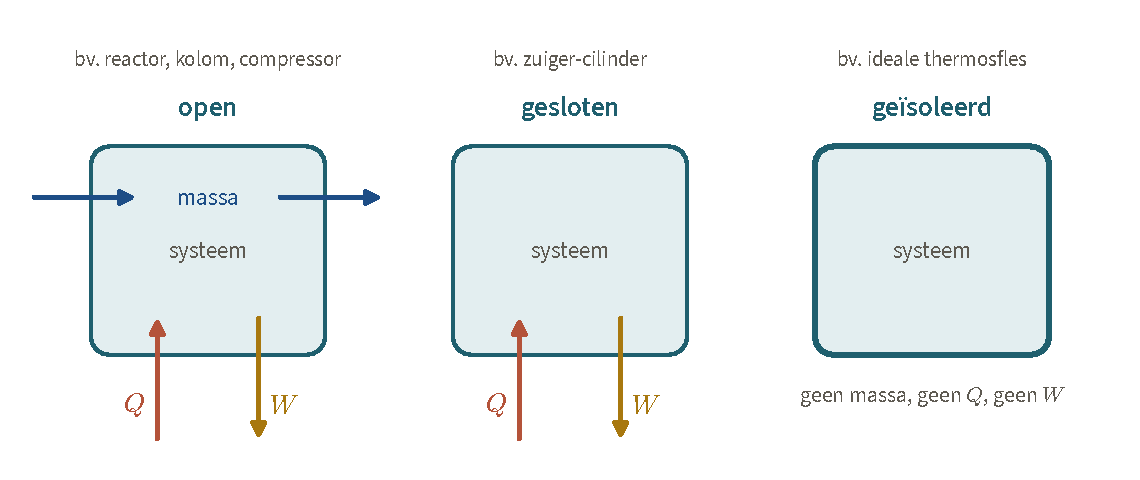
\includegraphics[width=0.9\linewidth]{Figuren/systemen}
    \caption{Open, gesloten, adiabatisch en ge\"isoleerd systeem. Een open systeem wisselt massa en energie uit, een gesloten systeem enkel energie (warmte $Q$ en arbeid $W$), een adiabatisch systeem enkel arbeid, een ge\"isoleerd systeem niets.}
    \label{fig:systemen}
\end{figure}

\begin{itemize}
\item Een \emph{gesloten systeem}, zoals gas in een zuiger-cilinder, wisselt geen massa uit, wel warmte en arbeid. De basiswetten leiden we eerst af voor gesloten systemen.
\item Een \emph{open systeem} laat ook massa door. Bijna elk industrieel toestel is open: pompen, compressoren, warmtewisselaars, kolommen, reactoren. De stromen voeren energie mee, en daarvoor zullen we de \emph{enthalpie} nodig hebben (\S~\ref{sec:enthalpie}).
\item Een \emph{adiabatisch systeem} heeft een grens die geen warmte doorlaat ($Q = 0$), maar wel arbeid. Dat gebeurt bij goede isolatie, maar ook als een proces zo snel verloopt dat er geen tijd is voor warmte-uitwisseling: de compressie in een fietspomp of dieselmotor, of een gas dat door een compressor stroomt. Alle arbeid blijft dan in het systeem en verhoogt de temperatuur (figuur~\ref{fig:compressie}). Hetzelfde geldt voor een goed ge\"isoleerde reactor, die opwarmt door zijn eigen reactiewarmte (\S~\ref{sec:warmte-effecten}). Adiabatisch zegt enkel iets over warmte: een adiabatisch systeem kan zowel open als gesloten zijn.
\item Een \emph{ge\"isoleerd systeem} wisselt helemaal niets uit. Het universum als geheel is het enige echte voorbeeld; een thermosfles of een calorimeter benadert het.
\end{itemize}


\section{Thermodynamisch evenwicht}

Een systeem laat zich pas eenduidig beschrijven als het in \emph{thermodynamisch evenwicht} is: na verloop van tijd zijn alle lokale verschillen in druk, temperatuur en samenstelling verdwenen. Daarvoor zijn drie voorwaarden nodig.
\begin{itemize}
\item \textbf{Thermisch evenwicht}: geen netto warmtestroom meer, dus overal dezelfde temperatuur.
\item \textbf{Mechanisch evenwicht}: geen netto kracht, bv.\ een zuiger staat stil als $p = p_\text{ext}$.
\item \textbf{Chemisch evenwicht}: de samenstelling verandert niet meer. Bij \ce{N2 + 3H2 <=> 2NH3} lopen heen- en terugreactie even snel; op moleculaire schaal gaat de reactie door, macroscopisch staat alles stil (\emph{dynamisch evenwicht}).
\end{itemize}

\begin{definitie}{Nulde hoofdwet van de thermodynamica}
Als systeem $A$ in thermisch evenwicht is met $C$, en $B$ ook met $C$, dan zijn $A$ en $B$ onderling in thermisch evenwicht.
\end{definitie}

Deze vanzelfsprekende uitspraak is de basis van elke temperatuurmeting: de thermometer speelt de rol van $C$.

\section{Toestandsvariabelen}

Een industri\"ele reactor van $100~\mathrm{m^3}$ bevat meer dan $10^{30}$ moleculen, maar zijn toestand ligt vast door enkele \emph{toestandsvariabelen}: druk, temperatuur, volume en samenstelling. We moeten dus niet de toestand van iedere molecule individueel bestuderen.

\subsection{Intensieve en extensieve grootheden}

Een \emph{extensieve grootheid} verdubbelt als je twee identieke systemen samenvoegt: massa $m$, volume $V$, hoeveelheid stof $n$, interne energie $U$, enthalpie $H$, entropie $S$. 

Een \emph{intensieve grootheid} hangt niet af van de grootte: temperatuur $T$, druk $p$, dichtheid $\rho$, concentratie, en elke molaire grootheid zoals $V_\mathrm{m} = V/n$. In een warmtewisselaar is het temperatuurverschil (intensief) de drijvende kracht, terwijl de overgedragen warmte (extensief) schaalt met het debiet.

\subsection{Toestandsfuncties en padfuncties}

Een \emph{toestandsfunctie} hangt enkel af van de toestand van het systeem, niet van de weg waarlangs die bereikt werd. De interne energie is er een voorbeeld hiervan: $\Delta U = U_2 - U_1$, welke weg je ook volgt. Hetzelfde geldt voor $H$, $S$ en $G$. Warmte en arbeid zijn daarentegen \emph{padfuncties}: hun waarde hangt af van het proces (figuur~\ref{fig:padfunctie}). Daarom schrijven we $\dd U$ (exacte differentiaal) maar $\delta Q$ en $\delta W$.

\begin{figure}[htb]
    \centering
    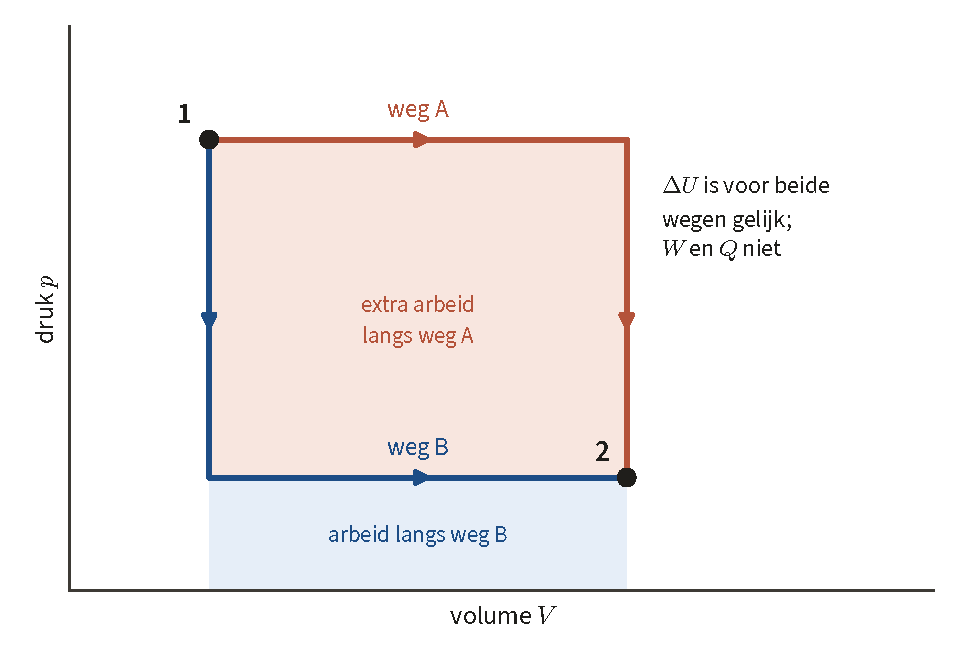
\includegraphics[width=0.7\linewidth]{Figuren/padfunctie}
    \caption{Twee wegen van toestand 1 naar toestand 2. De arbeid die het gas levert, is de oppervlakte onder de curve en is langs weg A veel groter. Omdat $\Delta U$ voor beide wegen gelijk is, moet ook de uitgewisselde warmte verschillen.}
    \label{fig:padfunctie}
\end{figure}

Je kan ook toepassen op zeer alledaagse situaties. Rij met de auto van een bergtop A naar het dal B en terug. De barometer toont in A voor en na de rit dezelfde druk: de luchtdruk is een toestandsfunctie. De brandstofmeter niet: hoeveel benzine je verbruikt hebt, hangt af van de gekozen route.


\section{Toestandsvergelijkingen}

Toestandsvariabelen zijn niet onafhankelijk: een \emph{toestandsvergelijking} verbindt ze. De eenvoudigste toestandsvergelijk is de ideale gaswet.

\subsection{De ideale gaswet}

Voor een verdund gas geldt
\begin{equation}
pV = nRT,
\end{equation}
met $R = \SI{8.314}{\joule\per\mole\per\kelvin}$ (in SI-eenheden; met bar en liter wordt dat \SI{0.08314}{\litre\bar\per\mole\per\kelvin}). De ideale gaswet is een \emph{limietwet}: elk gas voldoet aan deze toestandsvergelijk in de limiet $p \to 0$, en elke betere toestandsvergelijking moet in die limiet tot $pV = nRT$ herleiden.


\subsection{De ideale gaswet vanuit de moleculen: kinetische gastheorie}
\label{sec:kinetische-gastheorie}

De ideale gaswet werd experimenteel gevonden, maar ze laat zich ook afleiden uit een eenvoudig beeld van bewegende moleculen. Die afleiding is de moeite waard: ze toont wat druk en temperatuur op moleculair niveau \emph{betekenen}.

We maken drie aannames: 
\begin{enumerate}
    \item Het gas bestaat uit $N$ moleculen met massa $m$ die vrij en willekeurig door elkaar bewegen.
    \item De moleculen zelf nemen geen volume in.
    \item Er werken geen krachten tussen de moleculen; ze botsen enkel elastisch tegen de wand.
\end{enumerate}

De afleiding verloopt in drie stappen (figuur~\ref{fig:kmt-botsing}).

\begin{figure}[htb]
    \centering
    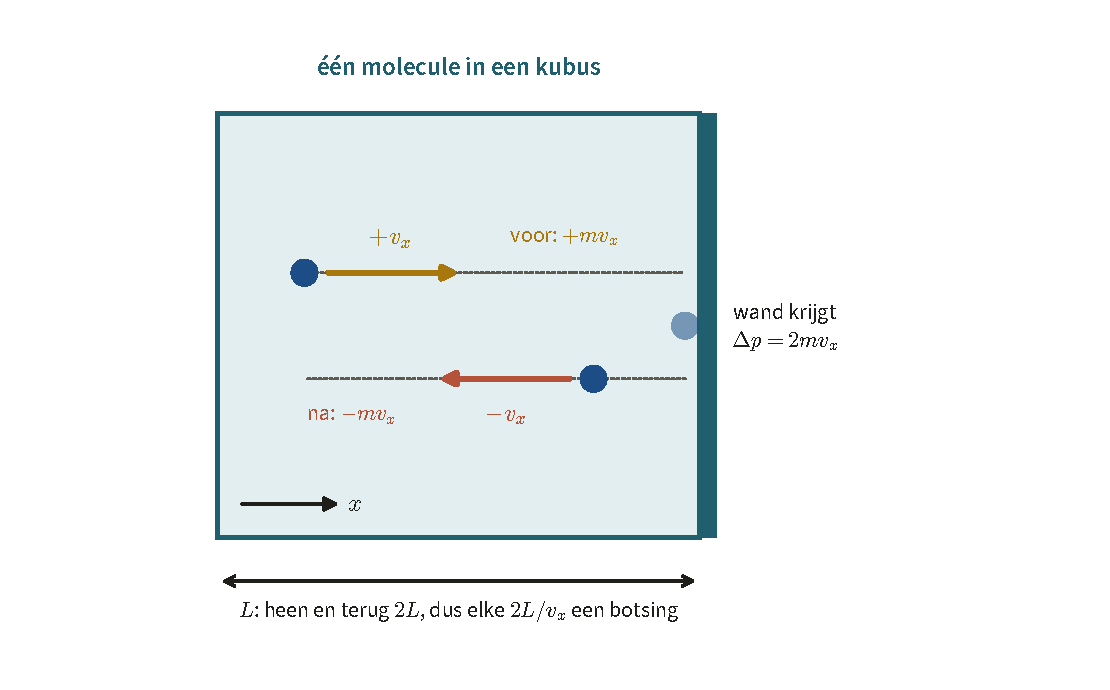
\includegraphics[width=0.85\linewidth]{Figuren/kmt_botsing}
    \caption{\'E\'en molecule in een kubus met ribbe $L$, die in de $x$-richting heen en weer beweegt. Bij elke botsing keert $v_x$ om en krijgt de wand een impuls $2mv_x$; na een heen-en-terugreis $2L$ komt de molecule terug.}
    \label{fig:kmt-botsing}
\end{figure}

\textbf{Stap 1: \'e\'en botsing.} Een molecule met snelheidscomponent $v_x$ botst elastisch tegen de wand loodrecht op $x$. Alleen $v_x$ keert om; $v_y$ en $v_z$ blijven gelijk. De impuls in de $x$-richting gaat van $+mv_x$ naar $-mv_x$, dus de wand krijgt een stoot $2mv_x$.

\textbf{Stap 2: hoe vaak?} Na de botsing moet de molecule naar de overkant en terug, een afstand $2L$. Dat duurt $2L/v_x$, dus ze botst $v_x/(2L)$ keer per seconde tegen dezelfde wand. De gemiddelde kracht van deze ene molecule is stoot maal frequentie:
\[
F_1 = 2mv_x \cdot \frac{v_x}{2L} = \frac{m v_x^2}{L}.
\]
Merk op dat $v_x$ hier \emph{twee keer} meetelt: een snellere molecule botst harder \'en vaker. Daarom verschijnt het kwadraat.

\textbf{Stap 3: alle moleculen samen.} Niet alle moleculen zijn even snel: sommige hebben een grote $v_x$, andere een kleine. We tellen de krachten van alle $N$ moleculen op en delen door de wandoppervlakte $L^2$. Met $L^3 = V$ wordt dat
\[
p = \frac{Nm\langle v_x^2\rangle}{V},
\]
met $\langle v_x^2\rangle$ het gemiddelde van $v_x^2$ over alle moleculen.

\paragraph{Waarom $\langle v^2\rangle$ en niet de gemiddelde snelheid?}
Je zou kunnen proberen te rekenen met \'e\'en ``gemiddelde'' snelheid, maar dat werkt niet. Het gemiddelde van $v_x$ zelf is nul: er bewegen evenveel moleculen naar links als naar rechts. Toch oefenen ze allemaal druk uit, elk op de wand waar ze naartoe vliegen. Wat telt is $v_x^2$, en dat is altijd positief. Het gemiddelde van een kwadraat is bovendien niet het kwadraat van een gemiddelde: wie $\langle v_x^2\rangle$ vervangt door $\langle |v_x|\rangle^2$, onderschat de druk, omdat de snelle moleculen in het kwadraat zwaarder doorwegen.

Rest nog de stap van $v_x$ naar de volledige snelheid. Voor elke molecule is $v^2 = v_x^2 + v_y^2 + v_z^2$ (Pythagoras). In een gas is geen enkele richting bevoordeeld (het gas is \emph{isotroop}), zodat de drie gemiddelden gelijk zijn: $\langle v_x^2\rangle = \langle v_y^2\rangle = \langle v_z^2\rangle = \tfrac{1}{3}\langle v^2\rangle$. Dus
\begin{equation}
pV = \tfrac{1}{3}\,N m \langle v^2\rangle .
\label{eq:kmt-druk}
\end{equation}
Druk is dus niets anders dan het gevolg van ontelbare kleine botsingen tegen de wand.

Vergelijken we dit met $pV = nRT$, dan volgt met $Nm = nM$ (molaire massa $M$):
\begin{equation}
\boxed{\tfrac{1}{2}M\langle v^2\rangle = \tfrac{3}{2}RT}
\qquad\text{of}\qquad
\boxed{v_\mathrm{rms} = \sqrt{\langle v^2\rangle} = \sqrt{\frac{3RT}{M}}}
\label{eq:vrms}
\end{equation}
De wortel uit het gemiddelde kwadraat heet de \emph{rms-snelheid} (root mean square). Ze is iets groter dan de gemiddelde snelheid $\bar v = \sqrt{8RT/\pi M}$, die we in hoofdstuk~\ref{ch:kinetiek} gebruiken voor botsingen tussen moleculen: $\bar v = 0.92\,v_\mathrm{rms}$. Voor de druk en de energie is $v_\mathrm{rms}$ de juiste grootheid, omdat beide met $v^2$ gaan. De temperatuur is dus een rechtstreekse maat voor de gemiddelde kinetische energie van de moleculen: $\tfrac{3}{2}RT$ per mol, of $\tfrac{3}{2}k_\mathrm{B}T$ per molecule. Voor een \'e\'enatomig ideaal gas is dat meteen de volledige interne energie, $U_\mathrm{m} = \tfrac{3}{2}RT$, zodat $C_{V,\mathrm{m}} = \tfrac{3}{2}R$ (zie \S~\ref{sec:warmtecapaciteiten}).

\begin{voorbeeld}{Hoe snel bewegen luchtmoleculen?}
Voor stikstof bij \SI{25}{\celsius} ($M = \SI{0.028}{\kilo\gram\per\mole}$):
\[
v_\mathrm{rms} = \sqrt{\frac{3(8.314)(298)}{0.028}} = \SI{515}{\metre\per\second}.
\]
Dat is sneller dan het geluid (\SI{346}{\metre\per\second}), wat logisch is: geluid wordt doorgegeven door botsende moleculen en kan dus niet sneller gaan dan de moleculen zelf. Helium ($M = \SI{0.004}{\kilo\gram\per\mole}$) is $\sqrt{28/4}\approx 2.6$ keer sneller: \SI{1360}{\metre\per\second}.

Toch ruik je een geopende parfumfles pas na enkele seconden aan de andere kant van de kamer. Een molecule vliegt immers niet rechtdoor: bij atmosferische druk botst ze ongeveer $10^{10}$ keer per seconde met andere moleculen. Botsingen tussen moleculen komen terug in hoofdstuk~\ref{ch:kinetiek}, waar ze de basis vormen van de reactiesnelheid.
\end{voorbeeld}

\begin{toepassing}{Effusie: de wet van Graham}
Wanneer een gas door een zeer klein gaatje ontsnapt (\emph{effusie}), is de snelheid waarmee dat gebeurt evenredig met de molecuulsnelheid, en dus met $1/\sqrt{M}$. Voor twee gassen bij dezelfde $T$ en $p$ geldt de \emph{wet van Graham}:
\begin{equation}
\frac{\text{effusiesnelheid A}}{\text{effusiesnelheid B}} = \sqrt{\frac{M_\mathrm{B}}{M_\mathrm{A}}}.
\end{equation}
\begin{itemize}
\item Een heliumballon loopt sneller leeg dan een luchtballon: helium ontsnapt $\sqrt{29/4}\approx 2.7$ keer sneller door de microporiën van het rubber.
\item Bij de verrijking van uranium wordt het verschil tussen \ce{^{235}UF6} en \ce{^{238}UF6} benut. De verhouding van de effusiesnelheden is slechts $\sqrt{352.0/349.0} = 1.0043$. Daarom waren duizenden diffusietrappen achter elkaar nodig; vandaag gebruikt men gascentrifuges.
\item Lekdetectie in vacu\"umsystemen gebeurt met helium: het lichte, snelle heliumatoom vindt zelfs de kleinste lekken.
\end{itemize}
\end{toepassing}

\subsection{Afwijkingen van ideaal gedrag}

Bij hoge druk en lage temperatuur gaan aannames (2) en (3) niet meer op. Dat zie je op drie manieren.
\begin{itemize}
\item \textbf{$pV$ is niet constant.} Volgens Boyle is $pV$ bij constante $T$ onafhankelijk van de druk (figuur~\ref{fig:Boyle}, links). Vergelijk je beide panelen van figuur~\ref{fig:Boyle}, dan zie je hoe groot de afwijking voor \ce{CO2} wordt: bij \SI{20}{\celsius} en \SI{0.5}{\litre\per\mole} voorspelt de ideale gaswet \SI{48.7}{\bar}, terwijl de werkelijke druk ongeveer \SI{37}{\bar} is, bijna een kwart lager. Voor een gas als stikstof bij kamertemperatuur blijft de afwijking onder \SI{10}{\bar} kleiner dan \SI{1}{\percent}, maar bij enkele honderden bar loopt ze op tot tientallen procenten.
\item \textbf{Joule--Thomson-effect.} Een gas dat zonder warmte-uitwisseling door een ventiel expandeert, koelt bij kamertemperatuur meestal af. Bij een ideaal gas zou $T$ constant blijven. De interne energie van een re\"eel gas hangt dus af van het volume: de moleculen trekken elkaar aan.
\item \textbf{Condensatie.} Volgens de ideale gaswet kan je een gas tot een willekeurig klein volume samenpersen. In werkelijkheid condenseert elk gas onder zijn \emph{kritische temperatuur} $T_c$ tot een vloeistof met een nagenoeg vast volume (figuur~\ref{fig:Boyle}, rechts). Boven $T_c$ (voor \ce{CO2} \SI{31.0}{\celsius}) condenseert het nooit, hoe hoog de druk ook wordt.
\end{itemize}

\begin{figure}[htb]
    \centering
    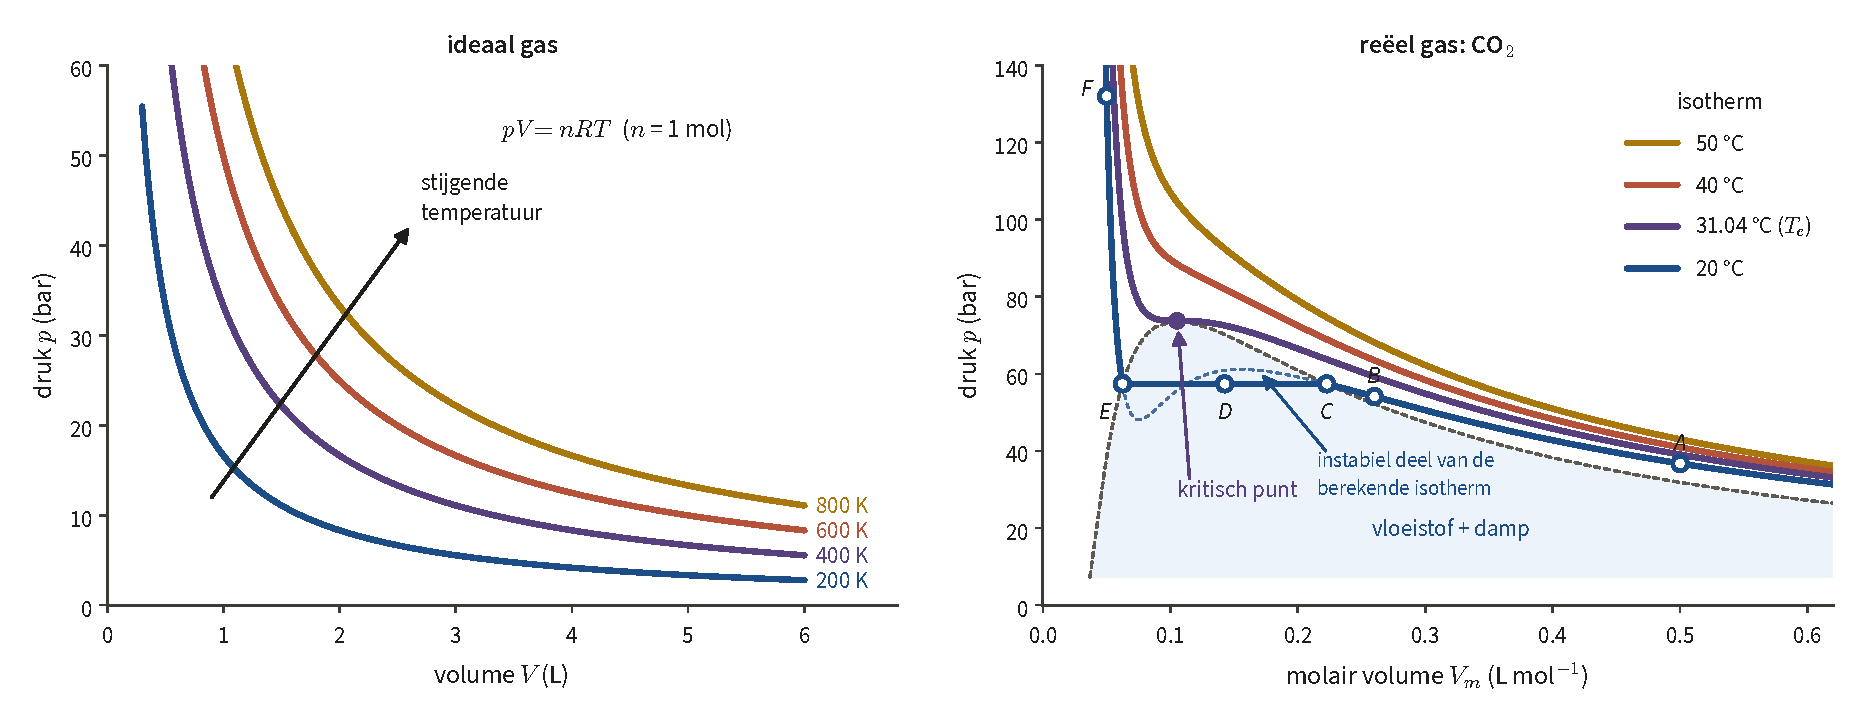
\includegraphics[width=\linewidth]{Figuren/isothermen_vergelijking}
    \caption{Isothermen van \ce{CO2} bij dezelfde temperaturen en op dezelfde assen. Links berekend met de ideale gaswet: $p \propto 1/V_m$ over het volledige bereik. Rechts het werkelijke gedrag (berekend met de toestandsvergelijking van Peng--Robinson, \S~\ref{sec:andere-toestandsvgl}). Bij groot molair volume liggen beide dicht bij elkaar; bij kleiner volume ligt de werkelijke druk lager. Onder de kritische temperatuur verschijnt een horizontaal stuk (C $\to$ E): daar condenseert het gas bij constante druk.}
    \label{fig:Boyle}
\end{figure}

\subsection{De vergelijking van Van der Waals}
\label{sec:vdw-afleiding}

Aannames (2) en (3) uit de ideale gaswet zijn niet exact: moleculen hebben wel een eigen volume en trekken elkaar wel aan. In 1873 corrigeerde Johannes Diderik van der Waals de ideale gaswet voor beide effecten, niet met een empirische fit maar vanuit hun fysische oorsprong. Hij verkreeg hiervoor de  Nobelprijs in 1910. Hieronder bespreken we zijn redenering in drie stappen.

\subsubsection{Stap 1: het uitgesloten volume}

\begin{figure}[htb]
    \centering
    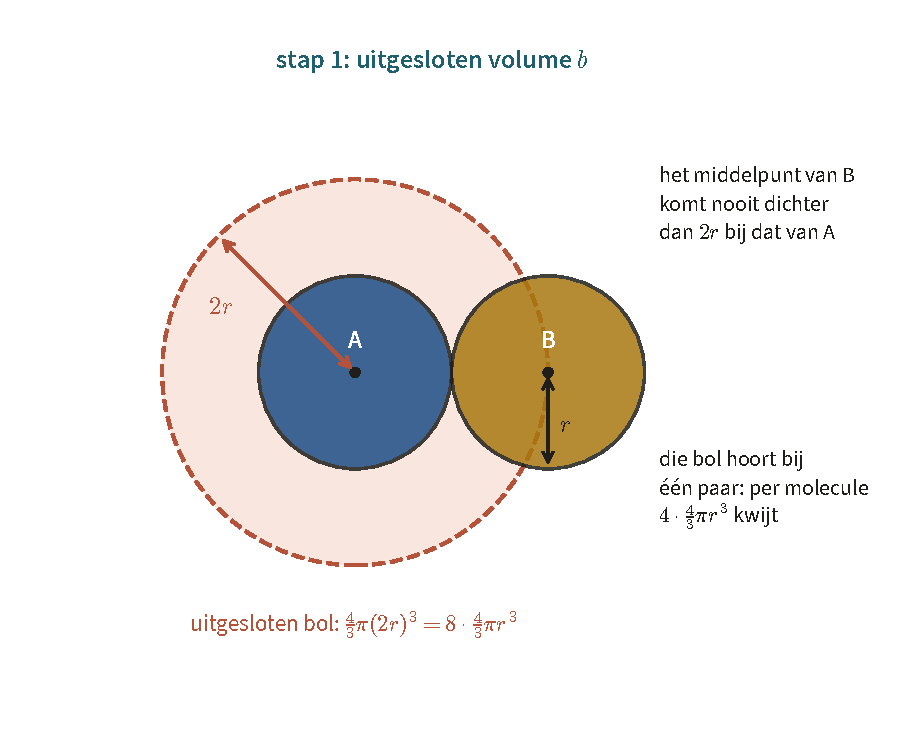
\includegraphics[width=0.6\linewidth]{Figuren/vdw_uitgesloten}
    \caption{Het uitgesloten volume. Rond molecule A ligt een bol met straal $2r$ waarin het middelpunt van B niet kan komen; dat volume is niet beschikbaar voor de beweging.}
    \label{fig:vdw-uitgesloten}
\end{figure}

Moleculen zijn geen puntmassa's (figuur~\ref{fig:vdw-uitgesloten}). Twee harde bollen met straal $r$ kunnen elkaars middelpunt niet dichter naderen dan $2r$. Rond elke molecule ligt dus een uitgesloten bol met volume $\tfrac{4}{3}\pi(2r)^3 = 8\cdot\tfrac{4}{3}\pi r^3$. Die bol is geen eigenschap van A alleen, maar van het paar A--B: hij beschrijft hoe dicht die twee elkaar kunnen naderen. Per molecule rekenen we hem dus maar half aan, zodat per molecule $4\cdot\tfrac{4}{3}\pi r^3$ is uitgesloten. Per mol is dat het \emph{co-volume} gelijk aan:
\begin{equation*}
b = 4 N_\mathrm{A} \cdot \tfrac{4}{3}\pi r^3 
\end{equation*}
Dit is viermaal het eigenlijke volume van de moleculen. Hierdoor is het vrije volume in de ruimte gelijk aan $V - nb$, en dus
\begin{equation}
p(V - nb) = nRT.
\end{equation}


\subsubsection{Stap 2: de drukcorrectie - intermoleculaire aantrekkingskrachten}

\begin{figure}[htb]
    \centering
    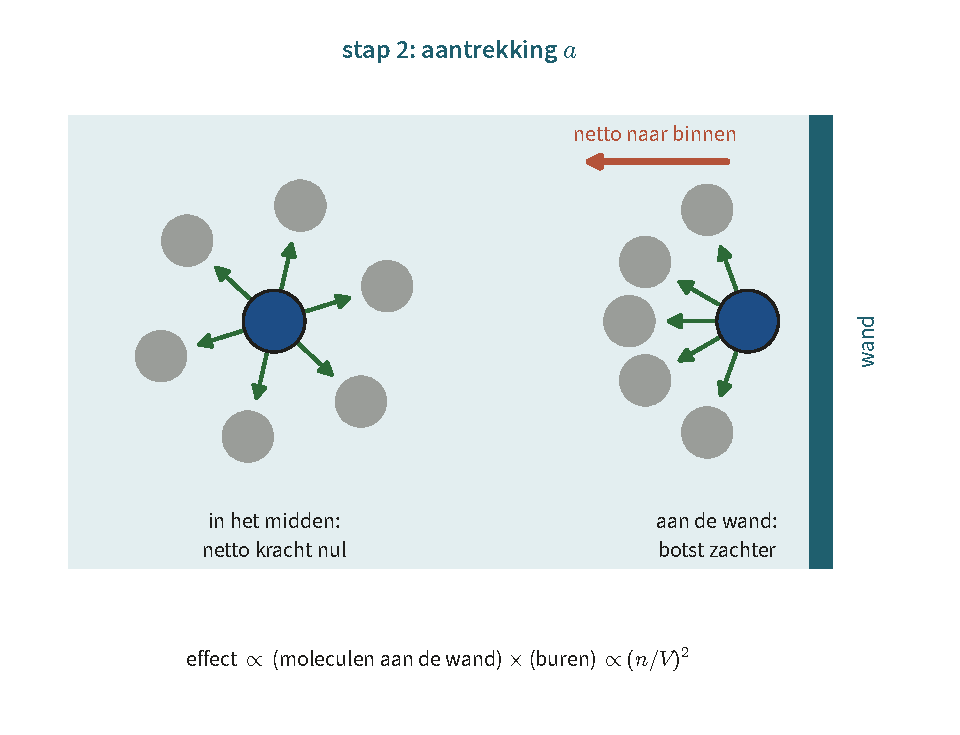
\includegraphics[width=0.65\linewidth]{Figuren/vdw_aantrekking}
    \caption{De aantrekking tussen moleculen. Een molecule in het midden van het gas wordt in alle richtingen even sterk aangetrokken, een molecule aan de wand enkel naar binnen. Ze botst daardoor zachter tegen de wand.}
    \label{fig:vdw-aantrekking}
\end{figure}

Reële moleculen trekken elkaar bovendien aan (figuur~\ref{fig:vdw-aantrekking}). Midden in het gas is een molecule langs alle kanten omringd door buren; hun aantrekkingskrachten heffen elkaar gemiddeld op. Een molecule die de wand nadert, heeft echter enkel nog buren aan de binnenkant en wordt dus netto teruggetrokken. Ze botst daardoor met een kleinere impuls tegen de wand, en de gemeten druk is lager dan bij een ideaal gas. Van der Waals schreef daarom
\begin{equation*}
p_{\mathrm{ideaal}} = p + p_{\mathrm{correctie}}.
\end{equation*}
Die correctie hangt af van het aantal paren moleculen dat elkaar aantrekt. Zowel het aantal moleculen nabij de wand als het aantal buren dat aan elk ervan trekt, is evenredig met de dichtheid $n/V$. De correctie is dus evenredig met het kwadraat: verdubbel je de dichtheid, dan wordt het effect vier keer groter.
\begin{equation}
p_{\mathrm{correctie}} = a\frac{n^2}{V^2}
\end{equation}
De stofconstante $a$ meet de sterkte van de aantrekking: groot voor \ce{CO2} en \ce{NH3}, klein voor He en \ce{H2}.

\subsubsection{Stap 3: combinatie van beide correcties}

Vervang in de ideale gaswet $p_{\mathrm{ideaal}} \to p + a n^2/V^2$ en $V_{\mathrm{ideaal}} \to V - nb$:
\begin{equation}
\boxed{\;\left(p + \frac{a n^2}{V^2}\right)(V - nb) = nRT\;}
\qquad\text{of per mol}\qquad
\boxed{\;\left(p + \frac{a}{V_m^2}\right)(V_m - b) = RT\;}
\label{eq:vdw}
\end{equation}

De parameters $a$ en $b$ zijn stofconstanten: je hoeft ze niet zelf te bepalen, maar zoekt ze op in tabellen. Tabel~\ref{tab:vdw-kort} geeft ze voor enkele veelgebruikte gassen; tabel~\ref{tab:kritiek} in bijlage~\ref{ch:tabellen} bevat een uitgebreidere lijst. De waarden tonen het fysische beeld van hierboven: kleine, apolaire moleculen (He, \ce{H2}) hebben een kleine $a$, polaire moleculen (\ce{NH3}, \ce{H2O}) en grotere moleculen (\ce{CO2}) een grote. De parameter $b$ volgt de grootte van de molecule.

\begin{table}[htb]
\centering
\caption{Van der Waals-parameters van enkele gassen, berekend uit de kritieke constanten met vergelijking~\eqref{eq:vdw-ab}. Bron kritieke constanten: zie tabel~\ref{tab:kritiek}.}
\label{tab:vdw-kort}
\begin{tabular}{lcc}
\toprule
gas & $a$ (\si{\pascal\metre\tothe{6}\per\mole\squared}) & $b$ ($10^{-5}$ \si{\metre\cubed\per\mole}) \\
\midrule
He & 0.0035 & 2.38 \\
\ce{H2} & 0.0248 & 2.66 \\
\ce{N2} & 0.137 & 3.86 \\
\ce{CH4} & 0.230 & 4.31 \\
\ce{CO2} & 0.366 & 4.29 \\
\ce{NH3} & 0.425 & 3.74 \\
\ce{H2O} & 0.553 & 3.05 \\
\bottomrule
\end{tabular}
\end{table}

\subsubsection{Het kritiek punt}

Een groot succes van de vergelijking is dat ze het \emph{kritiek punt} voorspelt. Wat is dat precies? Verwarm een vloeistof met haar damp in een gesloten, stevig vat. De vloeistof zet uit en wordt minder dicht; tegelijk verdampt er meer, zodat de damp erboven dichter wordt. Bij een bepaalde temperatuur worden beide dichtheden gelijk. Het scheidingsvlak (de meniscus) verdwijnt, en er is nog maar \'e\'en homogene fase. Die temperatuur is de \emph{kritieke temperatuur} $T_c$, de bijbehorende druk de \emph{kritieke druk} $p_c$ en het molair volume het \emph{kritieke volume} $V_{m,c}$.

Daaruit volgen twee praktische gevolgen:
\begin{itemize}
\item Boven $T_c$ kan je een gas \emph{niet} meer vloeibaar maken, hoe hoog je de druk ook opdrijft. Wie een gas wil vloeibaar maken (\ce{N2} of aardgas), moet het dus eerst onder $T_c$ afkoelen: voor stikstof onder \SI{126}{\kelvin}.
\item Boven $T_c$ \'en $p_c$ spreken we van een \emph{superkritisch fluïdum}. Het is zo dicht als een vloeistof en lost dus goed op, maar het stroomt en diffundeert als een gas. Superkritisch \ce{CO2} ($T_c = \SI{31}{\celsius}$, $p_c = \SI{74}{\bar}$) wordt zo gebruikt om cafe\"ine uit koffiebonen te extraheren, zonder resten van organische solventen.
\end{itemize}

Figuur~\ref{fig:vdw-isothermen} toont hoe de vergelijking van Van der Waals dit weergeeft. Boven $T_c$ daalt de druk monotoon met het volume: er is maar \'e\'en fase. Onder $T_c$ vertoont de isotherm een S-vormige lus. In werkelijkheid volgt het systeem die lus niet: het gas condenseert bij constante druk, langs het horizontale stuk (vergelijk met figuur~\ref{fig:Boyle}, rechts). Alle horizontale stukken samen vormen het tweefasengebied. Het kritiek punt is de top ervan: de isotherm bij $T_c$ is daar net horizontaal \'en verandert van kromming. Wiskundig is het dus een buigpunt met horizontale raaklijn:
\begin{equation*}
\left.\frac{\partial p}{\partial V_m}\right|_{T_c} = -\frac{RT_c}{(V_{m,c} - b)^2} + \frac{2a}{V_{m,c}^3} = 0,
\qquad
\left.\frac{\partial^2 p}{\partial V_m^2}\right|_{T_c} = \frac{2RT_c}{(V_{m,c} - b)^3} - \frac{6a}{V_{m,c}^4} = 0.
\end{equation*}

\begin{figure}[htb]
    \centering
    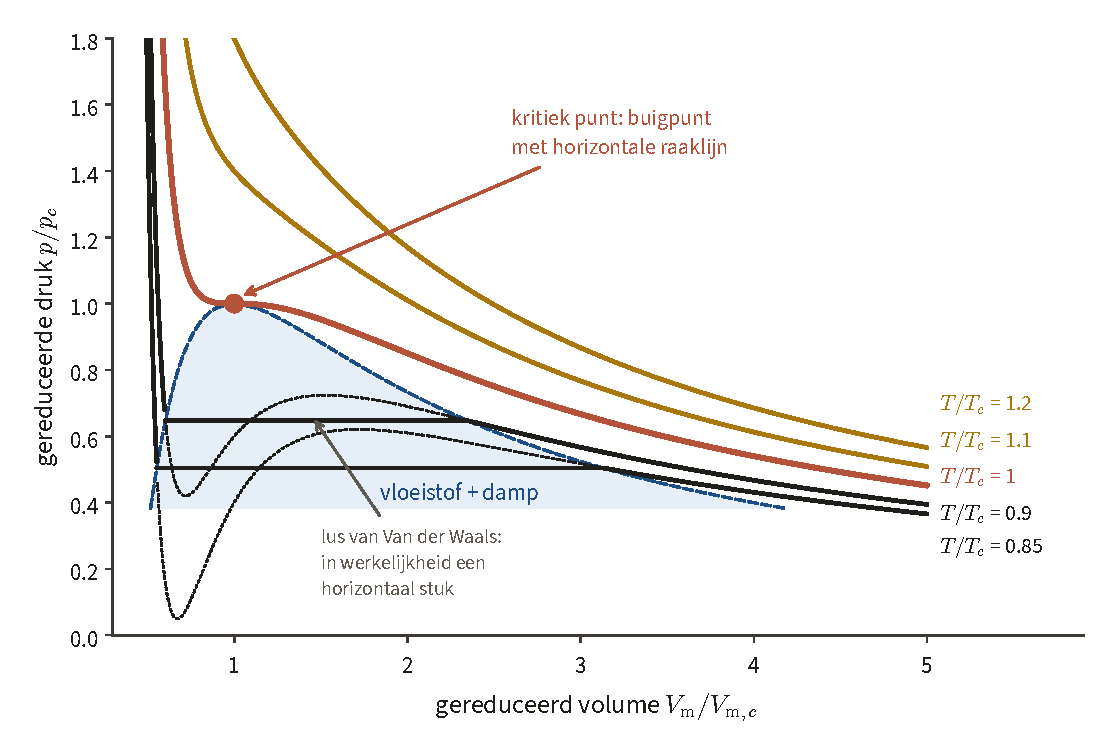
\includegraphics[width=0.85\linewidth]{Figuren/vdw_isothermen}
    \caption{Isothermen van Van der Waals in gereduceerde vorm ($p/p_c$ tegen $V_m/V_{m,c}$). Boven $T_c$ is er \'e\'en fase. Onder $T_c$ wordt de lus (stippellijn) in werkelijkheid vervangen door een horizontaal stuk: het gas condenseert bij constante druk. Het gekleurde gebied is het tweefasengebied, het kritiek punt de top ervan.}
    \label{fig:vdw-isothermen}
\end{figure}
Samen met de vergelijking zelf levert dit
\begin{equation}
V_{m,c} = 3b, \qquad T_c = \frac{8a}{27Rb}, \qquad p_c = \frac{a}{27b^2}
\qquad\Longleftrightarrow\qquad
a = \frac{27 R^2 T_c^2}{64 p_c}, \qquad b = \frac{R T_c}{8 p_c}.
\label{eq:vdw-ab}
\end{equation}
Zo bepaalt men $a$ en $b$ ook in de praktijk: de kritieke temperatuur en druk zijn nauwkeurig meetbaar, en daaruit volgen de parameters.

\begin{voorbeeld}{$a$ en $b$ voor $\mathrm{CO_2}$ uit het kritiek punt}
Met $T_c = \SI{304.2}{\kelvin}$ en $p_c = \SI{73.8}{\bar}$ (tabel~\ref{tab:kritiek}):
\begin{align*}
a &= \frac{27(8.314)^2(304.2)^2}{64(7.38\times10^{6})} = \SI{0.366}{\pascal\metre\tothe{6}\per\mole\squared},\\
b &= \frac{(8.314)(304.2)}{8(7.38\times10^{6})} = \SI{4.29e-5}{\metre\cubed\per\mole}.
\end{align*}
Dit zijn precies de waarden van tabel~\ref{tab:vdw-kort}: zo zijn die tabelwaarden ook berekend.
\end{voorbeeld}

\subsection{De compressibiliteitsfactor}

De afwijking wordt gemeten met de \emph{compressibiliteitsfactor}
\begin{equation}
\boxed{\;Z = \frac{V_\mathrm{m}}{V_\mathrm{m}^\text{ideaal}} = \frac{pV_\mathrm{m}}{RT}\;}
\end{equation}
Voor een ideaal gas is $Z = 1$. Bij $Z < 1$ is het gas compacter dan ideaal: de \emph{aantrekking} tussen de moleculen domineert (matige druk, lage $T$). Bij $Z > 1$ is het gas minder samendrukbaar: het \emph{eigen volume} van de moleculen domineert (zeer hoge druk). Voor $p \to 0$ of $T \to \infty$ gaat $Z \to 1$. Tabel~\ref{table:Z} en figuur~\ref{fig:Z} tonen dat verloop.

\begin{table}[htb]
\centering
\caption{Compressibiliteitsfactor $Z$ voor \ce{CO2} bij \SI{350}{\kelvin}.}
\label{table:Z}
\begin{tabular}{ccc}
\toprule
$p$ (\si{\bar}) & $V_\mathrm{m}$ (\si{\litre\per\mole}) & $Z$ \\
\midrule
1 & 24.5 & 1.00 \\
50 & 0.41 & 0.70 \\
200 & 0.15 & 1.03 \\
1000 & 0.045 & 2.16 \\
\bottomrule
\end{tabular}
\end{table}

\begin{figure}[htb]
    \centering
    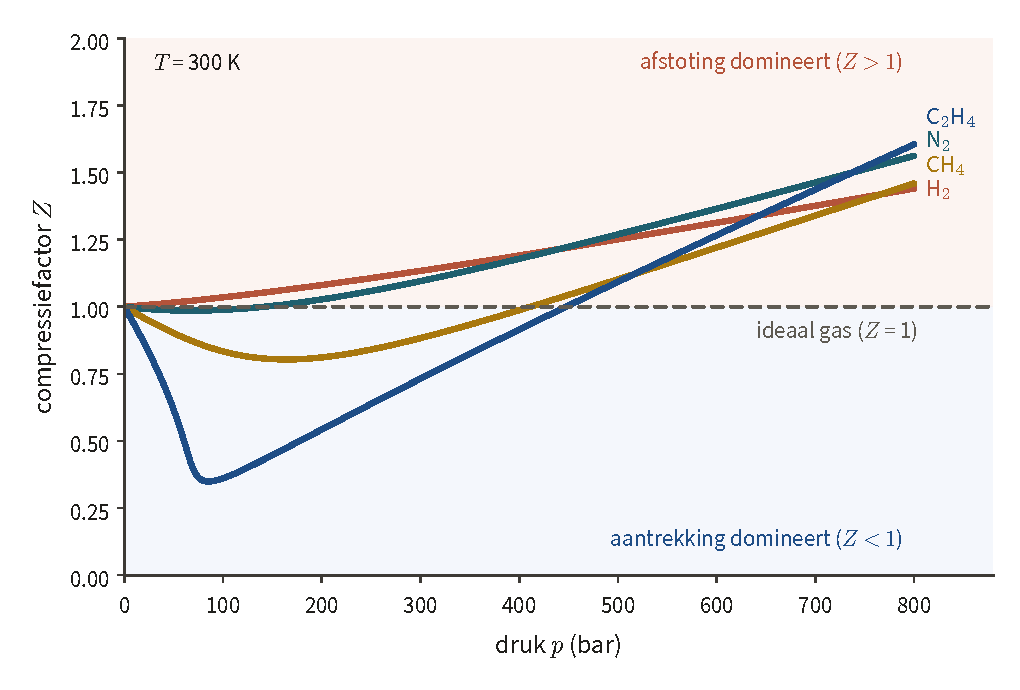
\includegraphics[width=0.7\linewidth]{Figuren/compressiefactor}
    \caption{Compressibiliteitsfactor in functie van de druk. Bij lage druk domineert de aantrekking ($Z<1$), bij hoge druk het eigen volume ($Z>1$).}
    \label{fig:Z}
\end{figure}

De vergelijking van Van der Waals verklaart beide richtingen. Je berekent $Z$ door eerst de druk uit vergelijking~\eqref{eq:vdw} te halen en die dan in de definitie van $Z$ in te vullen.

\begin{voorbeeld}{Vergelijking van het gedrag van \ce{CO2} en He}
We vergelijken beide gassen bij $T = \SI{300}{\kelvin}$ en $V_m = \SI{1.00e-3}{\metre\cubed\per\mole}$ (\SI{1.00}{\litre\per\mole}). De parameters $a$ en $b$ komen uit tabel~\ref{tab:vdw-kort}. Herschreven naar $p$ luidt de vergelijking van Van der Waals
\[
p = \frac{RT}{V_m - b} - \frac{a}{V_m^2},
\qquad\text{met}\qquad RT = (8.314)(300) = \SI{2494}{\joule\per\mole}.
\]
\textbf{Ideaal gas.} $p = RT/V_m = 2494/(1.00\times10^{-3}) = \SI{2.49}{\mega\pascal}$, en per definitie $Z = 1$.

\textbf{\ce{CO2}} ($a = \SI{0.366}{\pascal\metre\tothe{6}\per\mole\squared}$, $b = \SI{4.29e-5}{\metre\cubed\per\mole}$):
\begin{align*}
p &= \frac{2494}{1.00\times10^{-3} - 0.0429\times10^{-3}} - \frac{0.366}{(1.00\times10^{-3})^2}
   = \frac{2494}{0.957\times10^{-3}} - 0.366\times10^{6}\\
  &= 2.606\times10^{6} - 0.366\times10^{6} = \SI{2.24e6}{\pascal},\\
Z &= \frac{pV_m}{RT} = \frac{(2.24\times10^{6})(1.00\times10^{-3})}{2494} = 0.898.
\end{align*}
\textbf{He} ($a = \SI{0.0035}{\pascal\metre\tothe{6}\per\mole\squared}$, $b = \SI{2.38e-5}{\metre\cubed\per\mole}$):
\begin{align*}
p &= \frac{2494}{0.976\times10^{-3}} - \frac{0.0035}{(1.00\times10^{-3})^2}
   = 2.555\times10^{6} - 0.0035\times10^{6} = \SI{2.55e6}{\pascal},\\
Z &= \frac{(2.55\times10^{6})(1.00\times10^{-3})}{2494} = 1.023.
\end{align*}
Beide gassen wijken in tegengestelde richting af. Bij \ce{CO2} is de aantrekkingsterm groot ($a/V_m^2$ is ongeveer \SI{15}{\percent} van de druk): de aantrekking wint en $Z < 1$. Bij helium is de aantrekking verwaarloosbaar en verhoogt alleen het eigen volume de druk: $Z > 1$.
\end{voorbeeld}

Ook in het kritiek punt kan je $Z$ berekenen. Van der Waals voorspelt voor elk gas dezelfde waarde: met $V_{m,c} = 3b$, $T_c = 8a/(27Rb)$ en $p_c = a/(27b^2)$ volgt
\[
Z_c = \frac{p_c V_{m,c}}{RT_c} = \frac{3}{8} = 0.375.
\]
Gemeten waarden liggen lager en verschillen van stof tot stof: 0.301 (He), 0.290 (\ce{N2}), 0.274 (\ce{CO2}), 0.242 (\ce{NH3}) en 0.229 (\ce{H2O}) (tabel~\ref{tab:kritiek}). Van der Waals is dus kwalitatief juist, maar kwantitatief beperkt, vooral voor polaire stoffen.

Zet je $Z$ uit tegen de \emph{gereduceerde druk} $p_r = p/p_c$ bij een vaste \emph{gereduceerde temperatuur} $T_r = T/T_c$, dan vallen de curves van heel verschillende gassen nagenoeg samen (figuur~\ref{fig:compchart}). Dit is de \emph{wet van de corresponderende toestanden}. Ingenieurs gebruiken zulke algemene compressibiliteitskaarten wanneer geen specifieke toestandsvergelijking beschikbaar is.

\begin{figure}[htb]
    \centering
    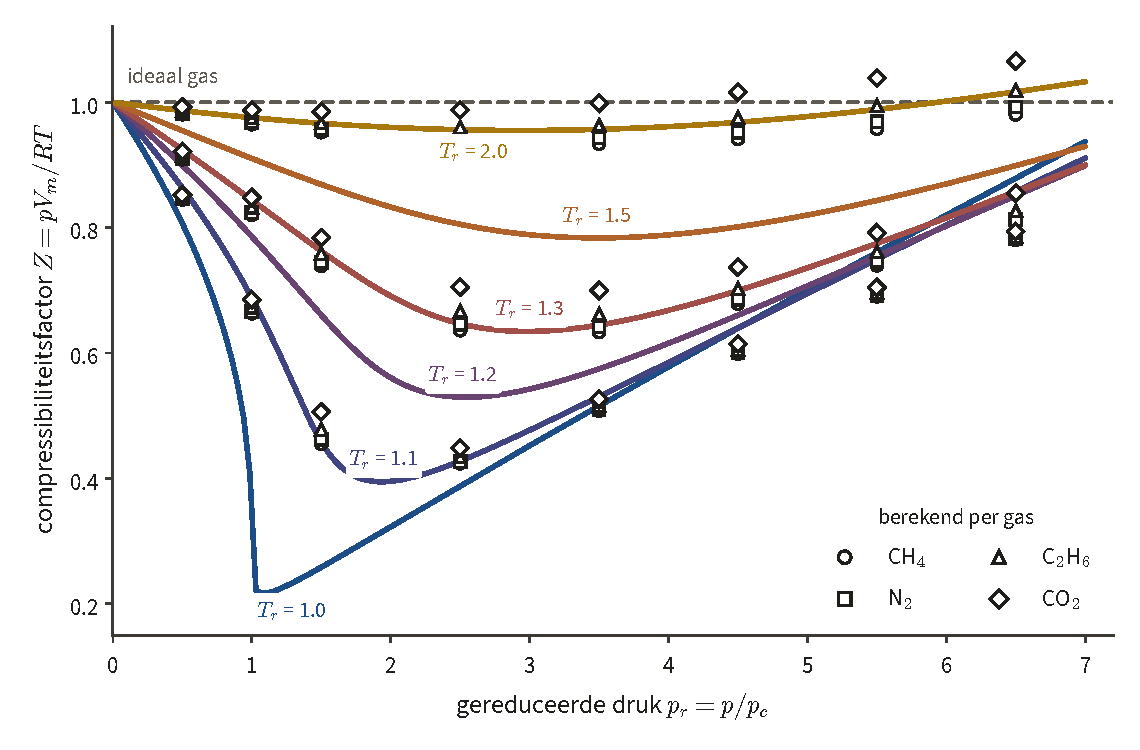
\includegraphics[width=0.7\linewidth]{Figuren/compressibiliteitskaart}
    \caption{Algemene compressibiliteitskaart: $Z$ tegen $p_r$ voor verschillende gassen bij dezelfde $T_r$.}
    \label{fig:compchart}
\end{figure}

\subsection{Andere toestandsvergelijkingen}
\label{sec:andere-toestandsvgl}

De vergelijking van Van der Waals schiet om drie redenen tekort: moleculen zijn geen harde bollen, de aantrekking $a$ hangt in werkelijkheid van de temperatuur af, en vloeistofdichtheden worden slecht voorspeld. Voor nauwkeurig ontwerpwerk gebruiken ingenieurs daarom andere toestandsvergelijkingen. Er zijn twee families.

\subsubsection{Kubische toestandsvergelijkingen}

Deze vergelijkingen behouden de structuur van Van der Waals, een afstotingsterm min een aantrekkingsterm, maar verfijnen beide. De belangrijkste zijn
\begin{align*}
\text{Redlich--Kwong (1949):}\quad & p = \frac{RT}{V_m - b} - \frac{a}{\sqrt{T}\,V_m(V_m + b)},\\
\text{Peng--Robinson (1976):}\quad & p = \frac{RT}{V_m - b} - \frac{a\,\alpha(T)}{V_m(V_m + b) + b(V_m - b)}.
\end{align*}
Soave--Redlich--Kwong (1972) vervangt in Redlich--Kwong de factor $1/\sqrt{T}$ door een functie $\alpha(T)$, zoals ook Peng--Robinson doet. Die $\alpha(T)$ hangt af van de \emph{acentrische factor} $\omega$, een getal uit tabellen dat meet hoe sterk een stof afwijkt van een eenvoudige, bolvormige molecule zoals argon. De parameters $a$ en $b$ volgen, net als bij Van der Waals, uit $T_c$ en $p_c$.

Ze heten \emph{kubisch} omdat ze, uitgewerkt naar $V_m$, een derdegraadsvergelijking opleveren. Onder de kritieke temperatuur ($T_c$) zijn die drie wortels: de kleinste is het molair volume van de vloeistof, de grootste dat van de damp, de middelste heeft geen fysische betekenis. Zo beschrijft \'e\'en vergelijking zowel de toestand van de gas- als vloeistoffase. Soave--Redlich--Kwong en Peng--Robinson zijn de standaard in processimulatoren zoals Aspen Plus en HYSYS; ook figuur~\ref{fig:Z} is met Peng--Robinson berekend.

\subsubsection{De viriaalvergelijking}

Een heel andere aanpak schrijft de afwijking van het ideaal gas als een machtreeks in $1/V_m$:
\begin{equation}
Z = \frac{pV_m}{RT} = 1 + \frac{B(T)}{V_m} + \frac{C(T)}{V_m^2} + \dots
\label{eq:viriaal}
\end{equation}
$B$ en $C$ heten de tweede en derde \emph{viriaalco\"effici\"ent}. Ze hangen enkel van de temperatuur af en worden per stof bepaald door de reeks te fitten op gemeten $p$-$V$-$T$-gegevens (tabel~\ref{tab:viriaal}).

\begin{table}[htb]
\centering
\caption{Tweede viriaalco\"effici\"ent $B$ (\si{\centi\metre\cubed\per\mole}).}
\label{tab:viriaal}
\begin{tabular}{lcc}
\toprule
gas & \SI{273}{\kelvin} & \SI{600}{\kelvin} \\
\midrule
He & 12.0 & 10.4 \\
\ce{N2} & $-10.5$ & 21.7 \\
Ar & $-21.7$ & 11.9 \\
\ce{CO2} & $-149.7$ & $-12.4$ \\
\bottomrule
\end{tabular}
\end{table}

Het teken van $B$ vertelt wat domineert. Een negatieve $B$ (\ce{CO2}, en \ce{N2} bij \SI{273}{\kelvin}) betekent $Z < 1$: de aantrekking wint. Bij hogere temperatuur wordt $B$ positief, omdat de moleculen dan zo snel bewegen dat de aantrekking weinig uitmaakt en enkel het eigen volume overblijft. De temperatuur waarbij $B = 0$ heet de \emph{Boyle-temperatuur}: daar gedraagt het gas zich bij lage druk opvallend ideaal.

De viriaalvergelijking is vooral een \emph{fitvergelijking}. Ze vertrekt niet van een fysisch beeld van de moleculen zoals Van der Waals, en de co\"effici\"enten volgen niet uit een theorie maar uit metingen. Dat is meteen haar sterkte: met genoeg termen beschrijft ze experimentele gegevens zo nauwkeurig als je wil. Bij lage tot matige dichtheid volstaat vaak de term in $B$ alleen. Haar zwakte is dat ze enkel geldt in het gebied waarop gefit werd: bij hoge dichtheid en in de buurt van condensatie convergeert de reeks niet meer, en een vloeistof beschrijft ze niet.

\section{Warmte en arbeid}

Tijdens compressie, expansie, opwarming of afkoeling wisselt een systeem energie uit met zijn omgeving. Dat kan op twee manieren: als \emph{arbeid} of als \emph{warmte}. Beide zijn padfuncties, maar ze verschillen fundamenteel van aard (figuur~\ref{fig:arbeid-warmte}).

\begin{figure}[htb]
    \centering
    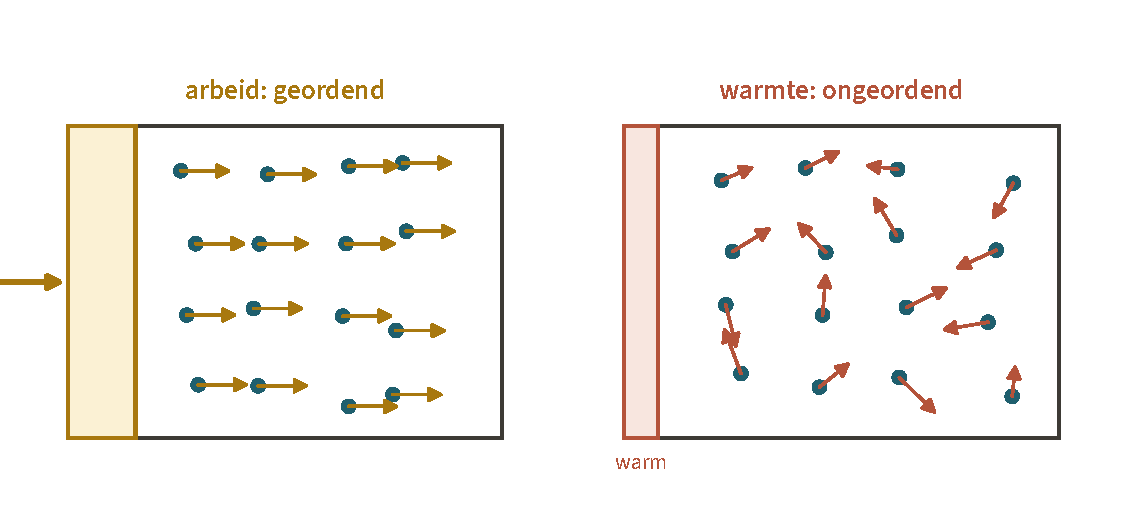
\includegraphics[width=0.85\linewidth]{Figuren/arbeid_warmte}
    \caption{Arbeid is geordende energieoverdracht: de zuiger geeft alle moleculen die hij raakt een duw in dezelfde richting. Warmte is ongeordend: een warme wand geeft moleculen een extra snelheid in willekeurige richtingen.}
    \label{fig:arbeid-warmte}
\end{figure}

\emph{Arbeid} is energieoverdracht door een macroscopische, gerichte kracht: een zuiger die een gas samendrukt, een gewicht dat wordt opgetild, elektronen die samen door een draad bewegen. Arbeid kan in principe volledig worden omgezet in een andere vorm van geordende energie. 

\emph{Warmte} is energieoverdracht die enkel door een temperatuurverschil wordt gedreven. De snelle moleculen van een warme wand stoten tegen de tragere gasmoleculen, die daarna in willekeurige richtingen sneller bewegen. Die wanorde maakt dat warmte niet volledig in arbeid kan worden omgezet; dat is het onderwerp van hoofdstuk~\ref{ch:spontaniteit}.

In chemische processen is de belangrijkste vorm van arbeid de \emph{volumearbeid}, verricht wanneer het volume verandert tegen een uitwendige druk:
\begin{equation}
\boxed{\;\delta W = -p_{\text{ext}}\,\dd V\;}
\end{equation}
We beschouwen energie die het systeem \emph{ontvangt} als positief. Bij expansie ($\dd V > 0$) levert het gas arbeid aan de omgeving, dus $W < 0$. In een $pV$-diagram is $|W|$ de oppervlakte onder de curve (figuur~\ref{fig:padfunctie}).

\begin{voorbeeld}{Arbeid bij isotherme expansie van een ideaal gas}
\SI{1}{\mole} ideaal gas expandeert reversibel en isotherm bij \SI{300}{\kelvin} van \SI{1}{\litre} naar \SI{10}{\litre}. Reversibel betekent $p_\text{ext} = p = nRT/V$, zodat
\[
W = -\int_{V_1}^{V_2} \frac{nRT}{V}\,\dd V = -nRT \ln\frac{V_2}{V_1} = -(1)(8.314)(300)\ln 10 = -\SI{5.74}{\kilo\joule}.
\]
Het gas levert \SI{5.74}{\kilo\joule} arbeid. Laat je het gas in \'e\'en ruk expanderen tegen de constante einddruk $p_\text{ext} = nRT/V_2 = \SI{2.49}{\bar}$, dan is $W = -p_\text{ext}\Delta V = -(2.49\times10^{5})(0.009) = -\SI{2.24}{\kilo\joule}$. Zelfde begin- en eindtoestand, minder dan de helft van de arbeid: arbeid hangt af van de weg.

Figuur~\ref{fig:arbeid-weg} maakt dat zichtbaar. De arbeid is de oppervlakte onder de weg in het $pV$-diagram. Bij de reversibele expansie volgt de uitwendige druk de gasdruk langs de isotherm, en die oppervlakte is groot. In \'e\'en ruk valt de uitwendige druk meteen naar $p_2$, en het gas duwt de hele weg tegen die lage druk: de oppervlakte is enkel de rechthoek onder $p_2$.

\begin{figure}[H]
    \centering
    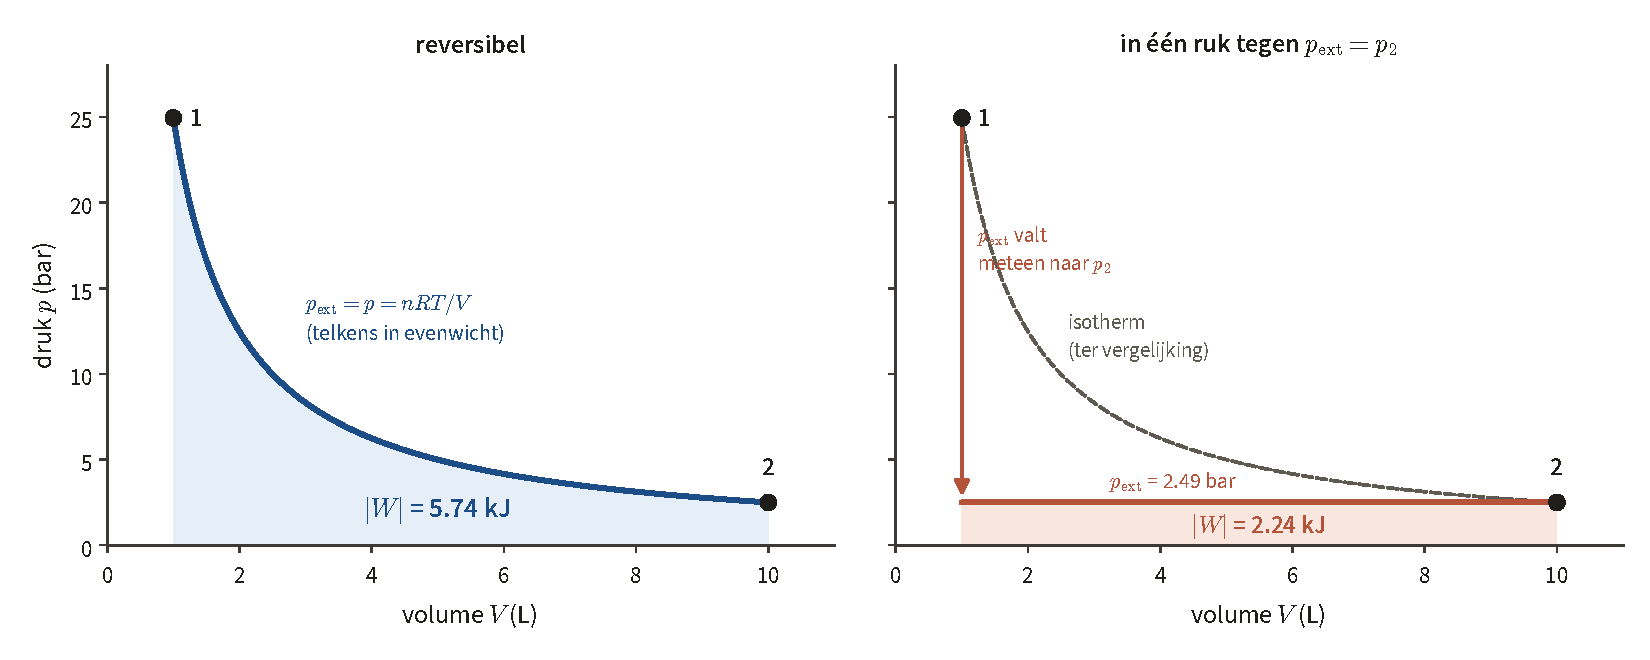
\includegraphics[width=\linewidth]{Figuren/arbeid_weg}
    \caption{Isotherme expansie van \SI{1}{\mole} ideaal gas van \SI{1}{\litre} naar \SI{10}{\litre} bij \SI{300}{\kelvin}. Links reversibel, rechts in \'e\'en ruk tegen $p_\text{ext} = p_2$. De gekleurde oppervlakte is $|W|$.}
    \label{fig:arbeid-weg}
\end{figure}

\textbf{Hoe doe je dit in de praktijk?} De reversibele isotherme expansie van links vraagt twee dingen tegelijk.
\begin{itemize}
\item \emph{Reversibel:} de uitwendige druk mag op elk ogenblik maar een fractie lager zijn dan de gasdruk. Het klassieke gedachte-experiment: belast een wrijvingsloze zuiger met een hoopje fijn zand en neem de korrels er \'e\'en voor \'e\'en af. Elke stap is een kleine expansie; hoe kleiner de stappen, hoe dichter de weg bij de isotherm ligt en hoe meer arbeid het gas levert.
\item \emph{Isotherm:} een gas dat arbeid levert, koelt af: het omgekeerde van de compressor die opwarmt (\S~\ref{sec:compressor}). Om $T$ constant te houden moet de omgeving tijdens de expansie warmte toevoeren, hier $Q = -W = \SI{5.74}{\kilo\joule}$. Dat lukt met een cilinder met dunne, goed geleidende wand in een groot thermostaatbad op \SI{300}{\kelvin}, en door zo traag te werken dat de warmte telkens kan bijbenen.
\end{itemize}
De vuistregel is dus: een proces is (bijna) isotherm als het veel trager verloopt dan de tijd die warmte nodig heeft om het gas te bereiken, en (bijna) adiabatisch als het veel sneller verloopt. Merk op dat ``isotherm'' alleen niet volstaat voor de maximale arbeid. Ook bij de expansie in \'e\'en ruk (rechts) kan het gas op het einde weer \SI{300}{\kelvin} hebben, maar de weg was niet reversibel.

Zuiver isotherm en reversibel bestaat in de industrie niet: het zou oneindig traag gaan. Wel benadert men het. Een gasexpander of stoomturbine wordt in trappen opgedeeld met \emph{tussenverwarming} ertussen, het spiegelbeeld van de tussenkoeling bij de compressor. Ook in de natuur zie je bijna isotherme expansie: een kleine luchtbel die in water opstijgt, verdubbelt van volume tussen \SI{10}{\metre} diepte en het oppervlak, maar blijft door het goede warmtecontact op watertemperatuur.
\end{voorbeeld}

\section{De eerste hoofdwet van de thermodynamica}

Energie ontstaat niet en verdwijnt niet; ze verandert enkel van vorm of wordt uitgewisseld. Om de energie \emph{in} een systeem te beschrijven, voeren we de \emph{interne energie} $U$ in. Ze omvat de translatie-, rotatie- en vibratie-energie van de moleculen, de potenti\"ele energie van de intermoleculaire krachten en de energie in chemische bindingen. De kinetische en potenti\"ele energie van het systeem als geheel tellen niet mee. $U$ is een toestandsfunctie.

\begin{definitie}{Eerste hoofdwet van de thermodynamica}
De verandering van de interne energie van een gesloten systeem is de som van de ontvangen warmte en de op het systeem verrichte arbeid:
\begin{equation}
\boxed{\dd U = \delta Q + \delta W}
\end{equation}
Met enkel reversibele volumearbeid wordt dit $\dd U = \delta Q - p\,\dd V$.
\end{definitie}

Bij een ideaal gas zijn er geen intermoleculaire krachten. De interne energie in dit geval is dus enkel de kinetische energie van de moleculen, en hangt enkel af van de temperatuur: $U = U(T)$ (\S~\ref{sec:kinetische-gastheorie}). Bij een re\"eel gas hangt $U$ ook af van de afstand tussen de moleculen, dus van het volume; dat is precies wat het Joule--Thomson-effect toont.

Een bekend gevolg merk je aan een fietspomp of een compressor: bij een snelle compressie wordt arbeid op het gas verricht ($W > 0$), terwijl er nauwelijks warmte weggaat ($Q \approx 0$). Dan is $\Delta U = W > 0$, en omdat $U$ van een (bijna) ideaal gas enkel van $T$ afhangt, stijgt de temperatuur. Hoeveel precies, werken we uit in \S~\ref{sec:compressor} zodra we de warmtecapaciteit kennen.

\begin{voorbeeld}{Arbeid bij isotherme compressie van een ideaal gas}
\SI{1}{\mole} ideaal gas wordt reversibel en isotherm gecomprimeerd bij \SI{300}{\kelvin} van \SI{1}{\bar} naar \SI{10}{\bar}. Omdat $T$ constant is, is $\Delta U = 0$: alle arbeid moet als warmte naar de omgeving. Met $V_2/V_1 = p_1/p_2$:
\[
W = -RT\ln\frac{V_2}{V_1} = RT\ln\frac{p_2}{p_1} = (8.314)(300)\ln 10 = \SI{5.74}{\kilo\joule\per\mole}, \qquad Q = -W.
\]
\end{voorbeeld}

\section{Enthalpie}
\label{sec:enthalpie}

In een open systeem, zoals een pomp, een turbine of een warmtewisselaar, stroomt materie in en uit. Dat in- en uitstromen kost arbeid. Bekijk een pakketje flu\"idum vlak v\'o\'or de inlaat van een toestel, in een leiding met doorsnede $A$ (figuur~\ref{fig:stromingsarbeid}). Het heeft druk $p_1$ en volume $V_1$, en dus lengte $L_1 = V_1/A$. Het pakketje gaat niet vanzelf naar binnen: het flu\"idum dat erop volgt (stroomopwaarts, links in de figuur) duwt het voor zich uit, net als een zuiger. Die denkbeeldige zuiger oefent een kracht $F = p_1A$ uit en verschuift het pakketje over zijn hele lengte $L_1$, tot het volledig in het toestel zit. De arbeid die zo aan het toestel geleverd wordt, is
\[
W_\text{in} = F\,L_1 = p_1A\cdot\frac{V_1}{A} = p_1V_1 .
\]
Aan de uitlaat gebeurt het omgekeerde. Het pakketje dat het toestel verlaat (druk $p_2$, volume $V_2$) moet het flu\"idum stroomafwaarts opzij duwen en levert daarbij arbeid $p_2V_2$ aan de omgeving. Elke stroom draagt dus naast zijn interne energie $U$ ook deze \emph{stromingsarbeid} $pV$ mee. Het is handig beide samen te nemen.

\begin{figure}[ht]
    \centering
    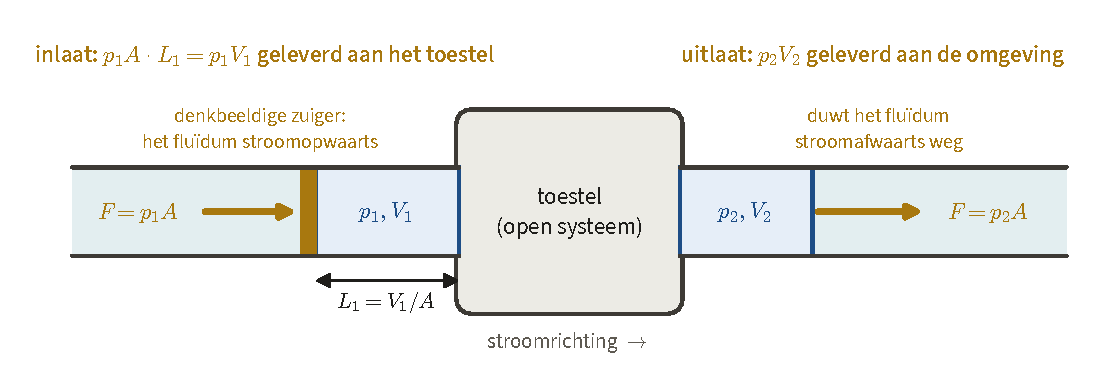
\includegraphics[width=\textwidth]{Figuren/stromingsarbeid}
    \caption{Stromingsarbeid. Aan de inlaat duwt het flu\"idum stroomopwaarts als een denkbeeldige zuiger een pakketje met kracht $p_1A$ over zijn lengte $L_1 = V_1/A$ naar binnen: het toestel ontvangt arbeid $p_1V_1$. Aan de uitlaat duwt het uittredende pakketje het flu\"idum stroomafwaarts weg: het toestel levert arbeid $p_2V_2$.}
    \label{fig:stromingsarbeid}
\end{figure}

\begin{definitie}{Enthalpie}
\begin{equation}
H = U + pV
\end{equation}
\end{definitie}

Differenti\"eren en de eerste hoofdwet invullen geeft $\dd H = \delta Q + V\,\dd p$. Bij \emph{constante druk} valt de laatste term weg:
\begin{equation}
\dd H = \delta Q_p .
\end{equation}
De enthalpieverandering is dus de warmte bij constante druk. Omdat de meeste processen bij (nagenoeg) constante druk lopen, rekenen ingenieurs bijna altijd met $H$: warmtewisselaars, kolommen en reactoren worden ontworpen met enthalpiebalansen. Voor vaste stoffen en vloeistoffen is $pV$ klein, zodat $\Delta H \approx \Delta U$; voor gassen is het verschil $\Delta(pV) = \Delta n_\text{gas}RT$.

Waar gaat dat verschil naartoe? Stel dat een reactie bij constante druk $p$ in een cilinder met een vrij bewegende zuiger loopt (figuren~\ref{fig:enthalpie-thermolyse} en~\ref{fig:enthalpie-vet}). Ontstaat er gas, dan schuift de zuiger op en duwt het systeem de atmosfeer weg: het levert arbeid $W = -p\,\Delta V$. Verdwijnt er gas, dan duwt de atmosfeer de zuiger in en krijgt het systeem arbeid. Met de ideale gaswet is $p\,\Delta V = \Delta n_\text{gas}RT$ (het volume van vaste stoffen en vloeistoffen verwaarlozen we), zodat de eerste hoofdwet $\Delta U = Q_p + W$ wordt
\begin{equation}
\Delta U = \Delta H - \Delta n_\text{gas}RT .
\label{eq:dU-dH}
\end{equation}
De warmte $Q_p = \Delta H$ en de verandering van de interne energie verschillen dus precies met de volumearbeid tegen de atmosfeer. Twee reacties uit het dagelijks leven tonen beide richtingen.

\begin{voorbeeld}{Thermolyse van kalksteen: warmte erin, arbeid eruit}
In een kalkoven wordt kalksteen ontbonden tot ongebluste kalk, de grondstof voor cement en mortel:
\[
\mathrm{CaCO_3(s)} \;\longrightarrow\; \mathrm{CaO(s)} + \mathrm{CO_2(g)}, \qquad \Delta H^\circ = +\SI{178.3}{\kilo\joule\per\mole} \quad (\SI{298}{\kelvin}).
\]
\begin{figure}[H]
    \centering
    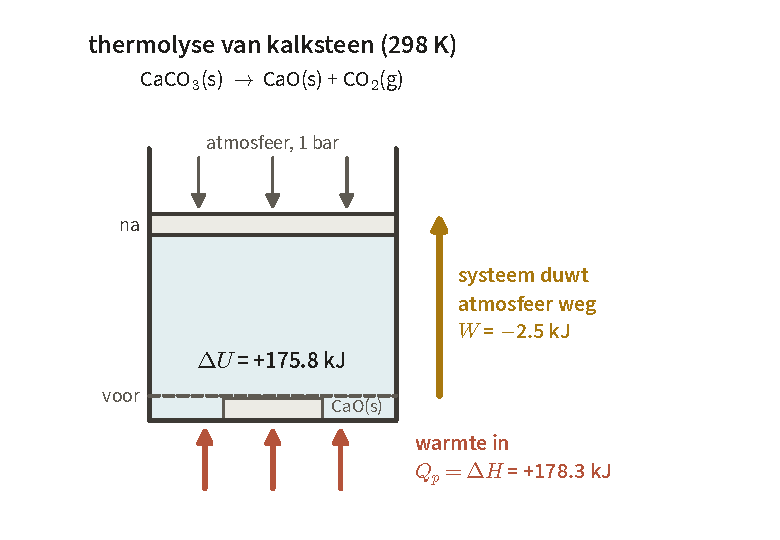
\includegraphics[width=0.75\textwidth]{Figuren/enthalpie_thermolyse}
    \caption{Thermolyse van kalksteen bij constante druk, per mol. Er ontstaat CO$_2$; de zuiger schuift op en een deel van de toegevoerde warmte verlaat het systeem weer als arbeid. Pijlen niet op schaal.}
    \label{fig:enthalpie-thermolyse}
\end{figure}
De reactie is endotherm: je moet \SI{178.3}{\kilo\joule} warmte toevoeren per mol. Er ontstaat \'e\'en mol gas uit niets dan vaste stof, dus $\Delta n_\text{gas} = +1$ en
\begin{align*}
W &= -\Delta n_\text{gas}RT = -(1)(8.314)(298) = \SI{-2.48}{\kilo\joule\per\mole},\\
\Delta U &= Q_p + W = 178.3 - 2.5 = \SI{175.8}{\kilo\joule\per\mole}.
\end{align*}
Van de toegevoerde warmte blijft dus \SI{175.8}{\kilo\joule} in het systeem (om de bindingen te herschikken) en lekt \SI{2.5}{\kilo\joule} weer weg als arbeid om de atmosfeer opzij te duwen voor het gevormde CO$_2$. In de oven, bij ongeveer \SI{900}{\celsius}, is die arbeid $RT \approx \SI{9.8}{\kilo\joule\per\mole}$: viermaal groter, maar nog steeds slechts enkele procent van de reactie-enthalpie.
\end{voorbeeld}

\begin{voorbeeld}{Verbranding van vet: warmte eruit, arbeid erin}
Je lichaam verbrandt vet, bijvoorbeeld tristearine, bij lichaamstemperatuur (\SI{310}{\kelvin}) en constante druk tot CO$_2$ en vloeibaar water:
\[
\mathrm{C_{57}H_{110}O_6(s)} + 81.5\,\mathrm{O_2(g)} \;\longrightarrow\; 57\,\mathrm{CO_2(g)} + 55\,\mathrm{H_2O(l)}, \qquad \Delta H \approx \SI{-35700}{\kilo\joule\per\mole}.
\]
\begin{figure}[H]
    \centering
    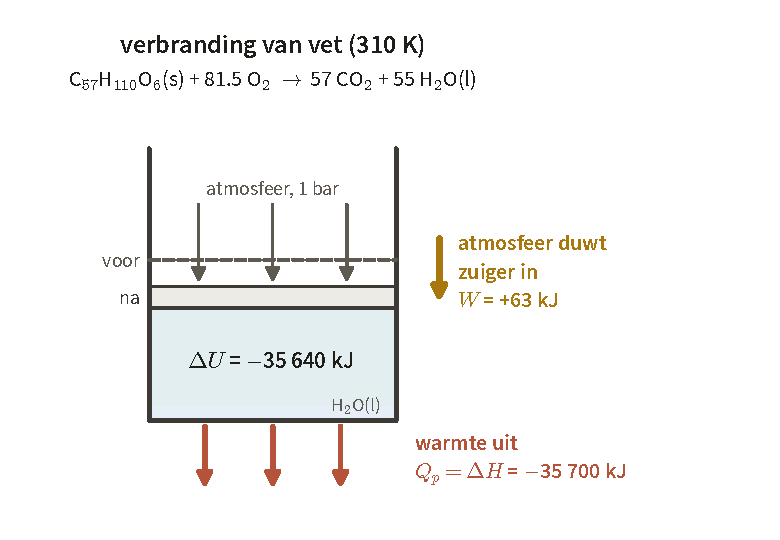
\includegraphics[width=0.75\textwidth]{Figuren/enthalpie_vet}
    \caption{Verbranding van tristearine bij constante druk, per mol. Er verdwijnt gas; de atmosfeer duwt de zuiger in en levert arbeid, zodat er meer warmte vrijkomt dan de interne energie daalt. Pijlen niet op schaal.}
    \label{fig:enthalpie-vet}
\end{figure}
Dat is ongeveer \SI{40}{\kilo\joule} per gram vet ($M = \SI{891.5}{\gram\per\mole}$). Hier \emph{verdwijnt} gas: $\Delta n_\text{gas} = 57 - 81.5 = -24.5$. De atmosfeer duwt het volume dus samen en levert arbeid aan het systeem:
\begin{align*}
W &= -\Delta n_\text{gas}RT = -(-24.5)(8.314)(310) = \SI{+63}{\kilo\joule\per\mole},\\
\Delta U &= Q_p + W = -35\,700 + 63 = \SI{-35640}{\kilo\joule\per\mole}.
\end{align*}
De vrijgekomen warmte ($|Q_p| = \SI{35700}{\kilo\joule}$) is dus \emph{groter} dan de daling van de interne energie ($\SI{35640}{\kilo\joule}$): de \SI{63}{\kilo\joule} arbeid die de omgeving levert, komt er als warmte bij. Er lekt hier niets weg; het is precies omgekeerd als bij de kalkoven. Het effect is klein (\SI{0.2}{\percent}), wat bevestigt dat $\Delta H \approx \Delta U$ voor de meeste reacties, maar het teken van $\Delta n_\text{gas}$ bepaalt in welke richting de arbeid loopt.
\end{voorbeeld}

\section{Warmtecapaciteiten}
\label{sec:warmtecapaciteiten}

Om een stof op te warmen is warmte nodig. De \emph{warmtecapaciteit} geeft aan hoeveel energie moet worden toegevoerd om de temperatuur van een systeem met \'e\'en kelvin te verhogen:
\begin{equation}
C = \frac{\dd Q}{\dd T}
\end{equation}

De \emph{warmtecapaciteit} is de warmte die nodig is om de temperatuur met \'e\'en kelvin te verhogen. Omdat warmte een padfunctie is, zijn er twee versies:
\begin{equation}
C_V = \left(\frac{\partial U}{\partial T}\right)_V
\qquad\qquad
C_p = \left(\frac{\partial H}{\partial T}\right)_p
\end{equation}
Bij constante druk zet het systeem bij opwarming uit en levert het arbeid, dus is meer warmte nodig: $C_p > C_V$. Hoeveel meer, volgt voor een ideaal gas rechtstreeks uit de definitie van enthalpie.

\begin{enumerate}
\item Vertrek van $H = U + pV$ en vul de ideale gaswet $pV = nRT$ in:
\[
H = U + nRT .
\]
\item Bij een ideaal gas oefenen de moleculen geen krachten op elkaar uit. De interne energie hangt dan enkel van de temperatuur af, niet van het volume of de druk: $U = U(T)$. Daardoor is ook $H = U(T) + nRT$ enkel een functie van $T$, en mag je de parti\"ele afgeleiden in de definities van $C_V$ en $C_p$ vervangen door gewone afgeleiden:
\[
C_V = \frac{\dd U}{\dd T}, \qquad C_p = \frac{\dd H}{\dd T}.
\]
\item Leid $H = U + nRT$ af naar $T$ ($n$ en $R$ zijn constant):
\[
\frac{\dd H}{\dd T} = \frac{\dd U}{\dd T} + nR
\qquad\Longrightarrow\qquad
C_p = C_V + nR .
\]
\item Deel door $n$ voor de molaire grootheden. Dat is de \emph{wet van Mayer}:
\begin{equation}
C_{p,\mathrm{m}} - C_{V,\mathrm{m}} = R .
\label{eq:mayer}
\end{equation}
\end{enumerate}
De term $nR$ heeft een eenvoudige betekenis: het is de arbeid die het gas per kelvin levert wanneer het bij constante druk uitzet, want $p\,\Delta V = nR\,\Delta T$. Voor \SI{1}{\mole} gas is dat \SI{8.314}{\joule} per kelvin, die je bij constante druk extra moet toevoeren bovenop wat naar de interne energie gaat. Voor vaste stoffen en vloeistoffen is de uitzetting zo klein dat $C_p \approx C_V$.
Een \'e\'enatomig gas heeft $C_{V,\mathrm{m}} = \tfrac{3}{2}R$ (enkel translatie); twee- en meeratomige gassen hebben meer, omdat ook rotatie en vibratie energie opnemen (\S~\ref{sec:moleculaire-beweging}).

\begin{voorbeeld}{Opwarmen van water versus lucht}
Om \SI{1}{\kilogram} op te warmen van \SI{20}{\celsius} naar \SI{30}{\celsius} heeft water ($c_p = \SI{4.18}{\kilo\joule\per\kilogram\per\kelvin}$) \SI{41.8}{\kilo\joule} nodig, lucht ($c_p = \SI{1.00}{\kilo\joule\per\kilogram\per\kelvin}$) slechts \SI{10.0}{\kilo\joule}. Per kilogram neemt water dus vier keer meer warmte op: daarom is het zo'n goede koelvloeistof.
\end{voorbeeld}

\subsection{Toepassing: waarom wordt een compressor warm?}
\label{sec:compressor}

Persluchtinstallaties, koelmachines en warmtepompen, de aardgastransportleiding: overal wordt gas gecomprimeerd. De gecomprimeerde lucht van een werkplaatscompressor verlaat de compressor gloeiend heet. Met de eerste hoofdwet en de warmtecapaciteit kunnen we nu berekenen hoe heet, en waarom dat ingenieurs zorgen baart.

\paragraph{Stap 1: de compressie is adiabatisch.}
Een gaspakketje doorloopt een compressor in een fractie van een seconde. Warmteoverdracht naar de wand is daarvoor veel te traag, zodat $Q \approx 0$. De eerste hoofdwet voor dat pakketje wordt dan $\dd U = \delta W = -p\,\dd V$: alle arbeid blijft als interne energie in het gas.

\paragraph{Stap 2: van arbeid naar temperatuur.}
Voor een ideaal gas is $\dd U = nC_{V,\mathrm{m}}\,\dd T$ en $p = nRT/V$. Invullen en scheiden van de veranderlijken geeft
\[
C_{V,\mathrm{m}}\,\frac{\dd T}{T} = -R\,\frac{\dd V}{V}
\qquad\Longrightarrow\qquad
\ln\frac{T_2}{T_1} = -\frac{R}{C_{V,\mathrm{m}}}\ln\frac{V_2}{V_1}.
\]
Het volume is in een compressor moeilijk te meten, de druk wel. Vervang daarom $V_2/V_1 = (T_2/T_1)(p_1/p_2)$ en gebruik $C_{V,\mathrm{m}} + R = C_{p,\mathrm{m}}$:
\begin{equation}
\boxed{\;\frac{T_2}{T_1} = \left(\frac{p_2}{p_1}\right)^{R/C_{p,\mathrm{m}}}\;}
\label{eq:adiabatische-compressie}
\end{equation}
De temperatuurstijging hangt dus enkel af van de \emph{drukverhouding}, niet van de absolute druk. Lucht bestaat uit tweeatomige moleculen met $C_{p,\mathrm{m}} \approx \tfrac{7}{2}R$, zodat $R/C_{p,\mathrm{m}} = 2/7 = 0.286$.

\paragraph{Stap 3: hoe warm?}
Lucht van \SI{20}{\celsius} wordt van \SI{1}{\bar} naar \SI{8}{\bar} gebracht, een gewone werkplaatsdruk:
\[
T_2 = (293.15)\,(8)^{0.286} = \SI{531}{\kelvin} = \SI{258}{\celsius}.
\]
Een re\"ele compressor heeft bovendien wrijving en verliezen, waardoor de lucht nog warmer wordt. Bij die temperatuur ontleedt smeerolie en vormt ze afzettingen, en in het ergste geval ontvlamt de oliedamp. De eindtemperatuur is daarom een harde ontwerpgrens.

\paragraph{Stap 4: hoeveel arbeid?}
Een compressor is een open systeem. Volgens \S~\ref{sec:enthalpie} is $\dd H = \delta Q + V\,\dd p$; zonder warmte-uitwisseling is de arbeid die de compressor per mol levert dus gelijk aan de enthalpiestijging van het gas:
\[
W_\text{adiabatisch} = \Delta H_\mathrm{m} = C_{p,\mathrm{m}}(T_2 - T_1) = \tfrac{7}{2}(8.314)(531 - 293) = \SI{6.92}{\kilo\joule\per\mole}.
\]
Zou je het gas tijdens de compressie perfect koelen (isotherm), dan is $W = \int V\,\dd p = RT\ln(p_2/p_1) = (8.314)(293)\ln 8 = \SI{5.07}{\kilo\joule\per\mole}$. De adiabatische compressie kost dus \SI{37}{\percent} meer arbeid. De reden zie je in $\int V\,\dd p$: het opgewarmde gas neemt bij elke druk een groter volume in, en dat volume moet de compressor verder samendrukken. In figuur~\ref{fig:compressie} is dat het gekleurde vlak tussen beide curven.

\paragraph{Stap 5: de oplossing is tussenkoeling.}
Perfect koelen tijdens de compressie lukt niet, maar je kan de compressie wel in stukken hakken. Een tweetrapscompressor brengt de lucht eerst van \SI{1}{\bar} naar \SI{2.83}{\bar} (drukverhouding $\sqrt{8}$), koelt ze in een \emph{tussenkoeler} terug tot \SI{20}{\celsius}, en comprimeert dan verder naar \SI{8}{\bar}. Elke trap haalt nu
\[
T = (293.15)\,(2.83)^{0.286} = \SI{395}{\kelvin} = \SI{121}{\celsius},
\]
en de totale arbeid daalt tot $2 \cdot \tfrac{7}{2}(8.314)(395 - 293) = \SI{5.90}{\kilo\joule\per\mole}$: \SI{15}{\percent} minder dan zonder tussenkoeling. De groene weg in figuur~\ref{fig:compressie} benadert de isotherm des te beter naarmate er meer trappen zijn. Daarom hebben compressoren voor hoge drukken, zoals die voor het vullen van duikflessen (\SI{200}{\bar}) of voor de ammoniaksynthese (150 tot \SI{300}{\bar}), drie tot vijf trappen met telkens een tussenkoeler.

\begin{figure}[htb]
    \centering
    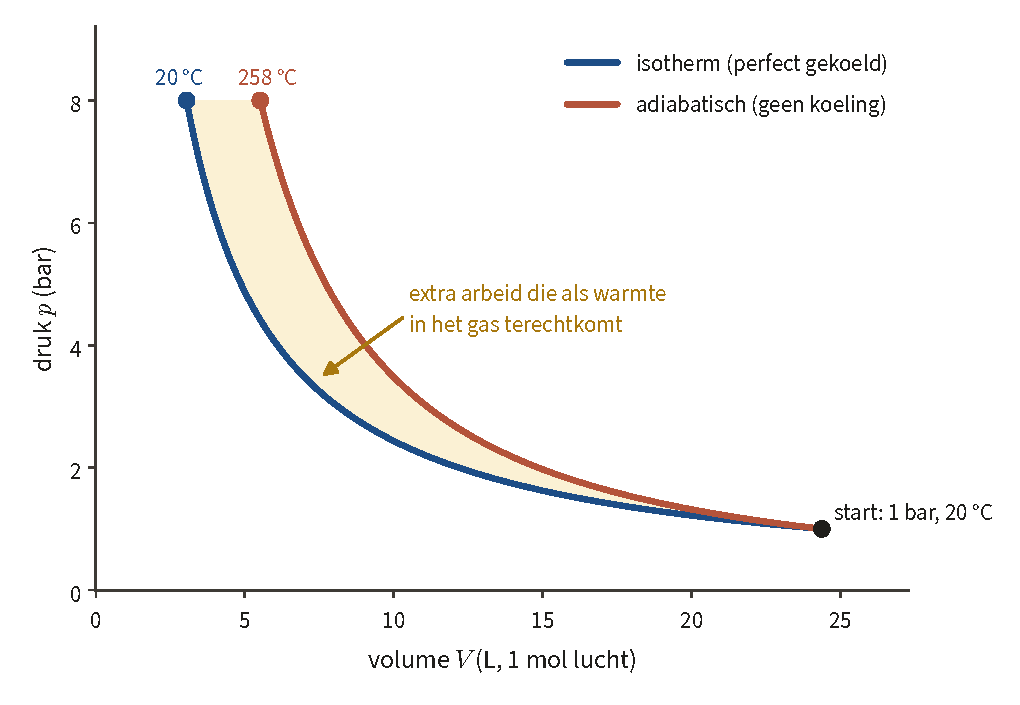
\includegraphics[width=0.75\linewidth]{Figuren/compressie_pv}
    \caption{Compressie van \SI{1}{\mole} lucht van \SI{1}{\bar} naar \SI{8}{\bar}, vertrekkend van \SI{20}{\celsius}. Isotherm: het gas wordt perfect gekoeld. Adiabatisch: alle arbeid blijft als interne energie in het gas. Tweetraps: adiabatisch tot \SI{2.83}{\bar}, terugkoelen tot \SI{20}{\celsius}, opnieuw adiabatisch. Het gekleurde vlak is de extra arbeid van de adiabatische compressie ten opzichte van de isotherme.}
    \label{fig:compressie}
\end{figure}

Hetzelfde effect benut men in een dieselmotor. Daar wordt lucht snel samengedrukt tot een twintigste van haar volume. Met vergelijking~\eqref{eq:adiabatische-compressie} herschreven naar volumes, $T_2/T_1 = (V_1/V_2)^{R/C_{V,\mathrm{m}}}$, loopt ze op van \SI{20}{\celsius} tot bijna \SI{700}{\celsius}, heet genoeg om de ingespoten diesel zonder bougie te ontsteken. Het omgekeerde voel je wanneer je lucht uit een fietsband laat ontsnappen: bij een snelle (adiabatische) expansie levert het gas arbeid, en daalt zijn temperatuur.



\section{Temperatuurafhankelijkheid van de enthalpie}

Bij opwarmen bij constante druk neemt de enthalpie toe volgens
\begin{equation}
\Delta H = \int_{T_1}^{T_2} C_p(T)\,\dd T \;\approx\; C_p\,(T_2-T_1) \quad\text{(als $C_p$ ongeveer constant is).}
\end{equation}
Over een groot temperatuurbereik is $C_p$ niet constant: hoe warmer, hoe meer vibraties worden aangeslagen, zodat $C_p$ stijgt (figuur~\ref{fig:cp-temperatuur}). Eenatomige gassen zoals helium hebben geen vibraties en dus een constante $C_p = \tfrac{5}{2}R$. Voor nauwkeurige berekeningen gebruikt men een empirische veelterm,
\begin{equation}
C_{p,\mathrm{m}} = a+bT+cT^2 ,
\end{equation}
met co\"effici\"enten zoals in tabel~\ref{tab:cp_coeff}. Processimulatoren (Aspen Plus, CHEMCAD) bevatten uitgebreide databanken van zulke correlaties.

\begin{figure}[htb]
    \centering
    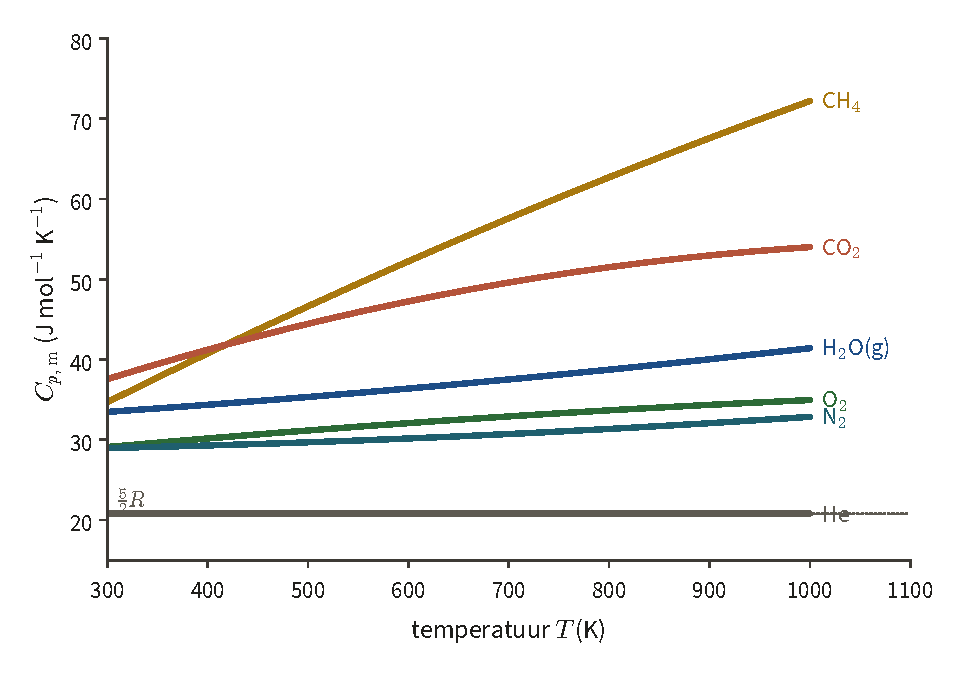
\includegraphics[width=0.7\linewidth]{Figuren/cp_temperatuur}
    \caption{Molaire warmtecapaciteit van enkele gassen tussen \SI{300}{\kelvin} en \SI{1000}{\kelvin} (correlaties uit tabel~\ref{tab:cp_coeff}, bron NIST). Hoe meer atomen, hoe meer vibraties en hoe sterker $C_p$ stijgt; helium blijft vlak op $\tfrac{5}{2}R$.}
    \label{fig:cp-temperatuur}
\end{figure}

\begin{table}[htb]
\centering
\caption{Benaderende co\"effici\"enten voor $C_{p,\mathrm{m}} = a + bT + cT^2$ (in \si{\joule\per\mole\per\kelvin}, $T$ in \si{\kelvin}), geldig tussen \SI{300}{\kelvin} en \SI{1000}{\kelvin} (afwijking kleiner dan \SI{1}{\joule\per\mole\per\kelvin}).
\label{tab:cp_coeff}
\begin{tabular}{lccc}
\toprule
Component & $a$ & $b$ & $c$ \\
\midrule
\ce{N2}     & 28.5 & $3.6\times10^{-4}$  & $4.00\times10^{-6}$ \\
\ce{O2}     & 25.4 & $1.35\times10^{-2}$ & $-3.95\times10^{-6}$ \\
Lucht       & 27.8 & $3.12\times10^{-3}$ & $2.33\times10^{-6}$ \\
\ce{H2}     & 29.1 & $-6.1\times10^{-4}$ & $1.65\times10^{-6}$ \\
\ce{CO}     & 27.7 & $3.12\times10^{-3}$ & $2.47\times10^{-6}$ \\
\ce{CO2}    & 23.9 & $5.21\times10^{-2}$ & $-2.20\times10^{-5}$ \\
\ce{CH4}    & 14.9 & $6.96\times10^{-2}$ & $-1.23\times10^{-5}$ \\
\ce{H2O(g)} & 31.3 & $5.99\times10^{-3}$ & $4.12\times10^{-6}$ \\
\ce{NH3}    & 24.4 & $3.86\times10^{-2}$ & $-6.40\times10^{-6}$ \\
He          & 20.8 & 0                   & 0 \\
\bottomrule
\end{tabular}
\end{table}

\begin{voorbeeld}{Enthalpieverandering van lucht}
Lucht wordt bij constante druk opgewarmd van \SI{300}{\kelvin} naar \SI{600}{\kelvin}. Term per term integreren:
\begin{align*}
\Delta H_\mathrm{m} &= a(T_2-T_1) + \frac{b}{2}(T_2^2-T_1^2) + \frac{c}{3}(T_2^3-T_1^3)\\
&= 27.8(300) + \frac{3.12\times10^{-3}}{2}(600^2-300^2) + \frac{2.33\times10^{-6}}{3}(600^3-300^3)\\
&= 8350 + 421 + 147 = \SI{8.92}{\kilo\joule\per\mole}.
\end{align*}
Met een constante $C_{p,\mathrm{m}} = \SI{29.7}{\joule\per\mole\per\kelvin}$ (de waarde bij \SI{450}{\kelvin}, halfweg) vind je \SI{8.90}{\kilo\joule\per\mole}; met de waarde bij \SI{300}{\kelvin} (\SI{29.0}{\joule\per\mole\per\kelvin}) \SI{8.70}{\kilo\joule\per\mole}, nog geen \SI{3}{\percent} te weinig. Een gemiddelde $C_p$ volstaat dus vaak; de veelterm wordt belangrijk bij grote temperatuursprongen, zoals in een vlam (\S~\ref{sec:warmte-effecten}).
\end{voorbeeld}

\section{Standaardtoestanden en de wet van Hess}
\label{sec:hess}

Enthalpie\"en worden altijd opgegeven ten opzichte van een \emph{standaardtoestand}: zuivere stof bij \SI{1}{\bar}, meestal getabelleerd bij \SI{298.15}{\kelvin}. De \emph{standaardvormingsenthalpie} $\Delta H_f^\circ$ is de enthalpieverandering wanneer \'e\'en mol van een stof gevormd wordt uit de elementen in hun standaardtoestand. Voor die elementen zelf is $\Delta H_f^\circ = 0$. Omdat $H$ een toestandsfunctie is, mag je elke reactie opsplitsen in ``ontbinden tot elementen'' en ``opbouwen tot producten'' (figuur~\ref{fig:hess}). Dat is de \emph{wet van Hess}:
\begin{equation}
\Delta_r H^\circ = \sum_i \nu_i\, \Delta H_{f,i}^\circ ,
\end{equation}
met $\nu_i$ positief voor producten en negatief voor reagentia. Op dezelfde manier worden standaardentropie\"en $S^\circ$ en vormings-Gibbsenergie\"en $\Delta G_f^\circ$ getabelleerd (hoofdstuk~\ref{ch:spontaniteit}).

\begin{figure}[htb]
    \centering
    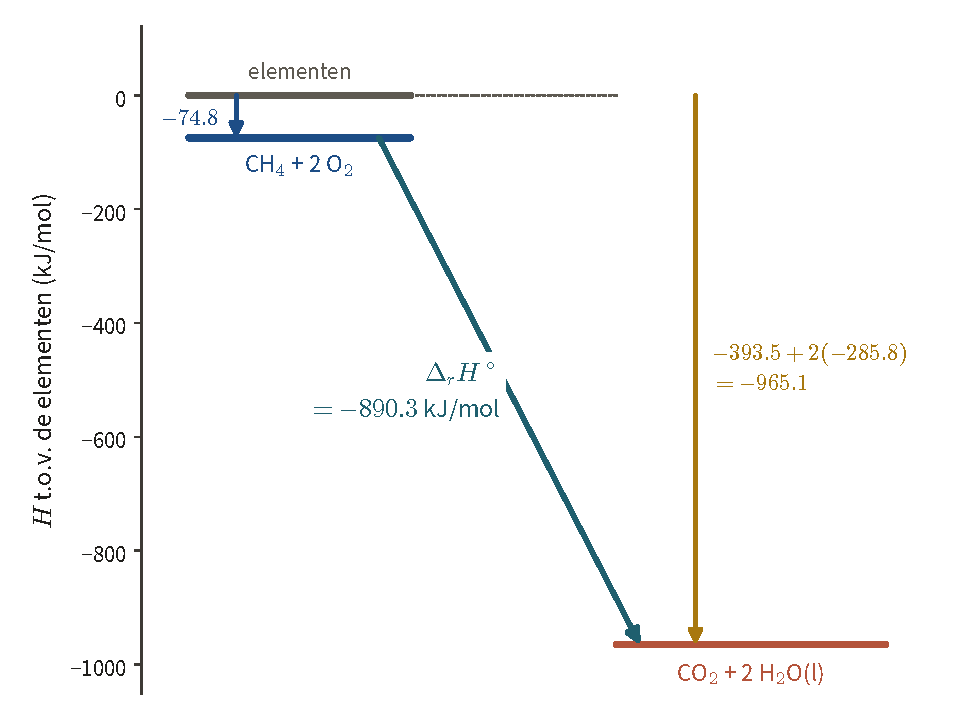
\includegraphics[width=0.7\linewidth]{Figuren/hess}
    \caption{Enthalpiediagram voor de verbranding van methaan. De elementen liggen per definitie op nul. De reactie-enthalpie is het verschil tussen het niveau van de producten en dat van de reagentia, welke weg je ook volgt.}
    \label{fig:hess}
\end{figure}

\begin{voorbeeld}{Reactie-enthalpie via de wet van Hess}
Voor \ce{CH4(g) + 2 O2(g) -> CO2(g) + 2 H2O(l)} met $\Delta H_f^\circ$ = $-74.8$ (\ce{CH4}), $-393.5$ (\ce{CO2}) en $-285.8$ (\ce{H2O(l)}) \si{\kilo\joule\per\mole}:
\[
\Delta_r H^\circ = (-393.5) + 2(-285.8) - (-74.8) = \SI{-890.3}{\kilo\joule\per\mole}.
\]
Per mol methaan komt \SI{890.3}{\kilo\joule} vrij: de basis voor het ontwerp van elke aardgasbrander.
\end{voorbeeld}

\section{Temperatuurafhankelijkheid van reactie-enthalpie\"en: de wet van Kirchhoff}
\label{sec:kirchhoff}

Tabellen geven reactie- en vormingsenthalpie\"en bij \SI{298}{\kelvin}, maar reacties lopen zelden bij kamertemperatuur. Ammoniak wordt gemaakt bij ongeveer \SI{450}{\celsius}, methanol bij \SI{250}{\celsius}, kalk bij \SI{900}{\celsius}. Hoe reken je de reactie-enthalpie om naar de procestemperatuur?

\paragraph{Afleiding met een kringloop.} Omdat $H$ een toestandsfunctie is, mag je van reagentia bij $T_0 = \SI{298}{\kelvin}$ naar producten bij een andere temperatuur $T$ gaan langs elke weg die je wil. Vergelijk twee wegen:
\begin{enumerate}
\item \emph{Eerst reageren, dan opwarmen.} Laat de reactie verlopen bij $T_0$ en warm daarna de producten op van $T_0$ tot $T$:
\[
\Delta H_\text{weg 1} = \Delta_r H^\circ(T_0) + \int_{T_0}^{T} C_{p,\text{producten}}\,\dd T .
\]
\item \emph{Eerst opwarmen, dan reageren.} Warm de reagentia op van $T_0$ tot $T$ en laat de reactie daar verlopen:
\[
\Delta H_\text{weg 2} = \int_{T_0}^{T} C_{p,\text{reagentia}}\,\dd T + \Delta_r H^\circ(T) .
\]
\item Begin- en eindtoestand zijn dezelfde, dus $\Delta H_\text{weg 1} = \Delta H_\text{weg 2}$. Oplossen naar $\Delta_r H^\circ(T)$ geeft de \emph{wet van Kirchhoff}:
\begin{equation}
\boxed{\;\Delta_r H^\circ(T) = \Delta_r H^\circ(T_0) + \int_{T_0}^{T} \Delta_r C_p^\circ\,\dd T\;}
\label{eq:kirchhoff}
\end{equation}
met
\[
\Delta_r C_p^\circ = \sum_\text{producten} \nu\, C_{p,\mathrm{m}}^\circ - \sum_\text{reagentia} \nu\, C_{p,\mathrm{m}}^\circ .
\]
\end{enumerate}
In differentiaalvorm staat er $\dd(\Delta_r H^\circ)/\dd T = \Delta_r C_p^\circ$: de reactie-enthalpie verandert met de temperatuur precies zo snel als het verschil in warmtecapaciteit tussen producten en reagentia.

\paragraph{Grafisch.} Teken de enthalpie van de reagentia en van de producten als functie van $T$ (figuur~\ref{fig:kirchhoff}, links). Elke lijn stijgt met een helling gelijk aan de totale warmtecapaciteit, en de verticale afstand tussen beide lijnen is $\Delta_r H^\circ(T)$. De twee wegen uit de afleiding zijn de twee manieren om van het blauwe punt linksboven naar het rode punt rechtsonder te gaan: eerst omlaag en dan langs de rode lijn, of eerst langs de blauwe lijn en dan omlaag. Lopen de lijnen evenwijdig ($\Delta_r C_p = 0$), dan hangt $\Delta_r H$ niet van de temperatuur af. Hebben de reagentia de grotere warmtecapaciteit, zoals bij de ammoniaksynthese, dan gaan de lijnen uit elkaar en wordt de reactie bij hogere temperatuur sterker exotherm.

\begin{figure}[htb]
    \centering
    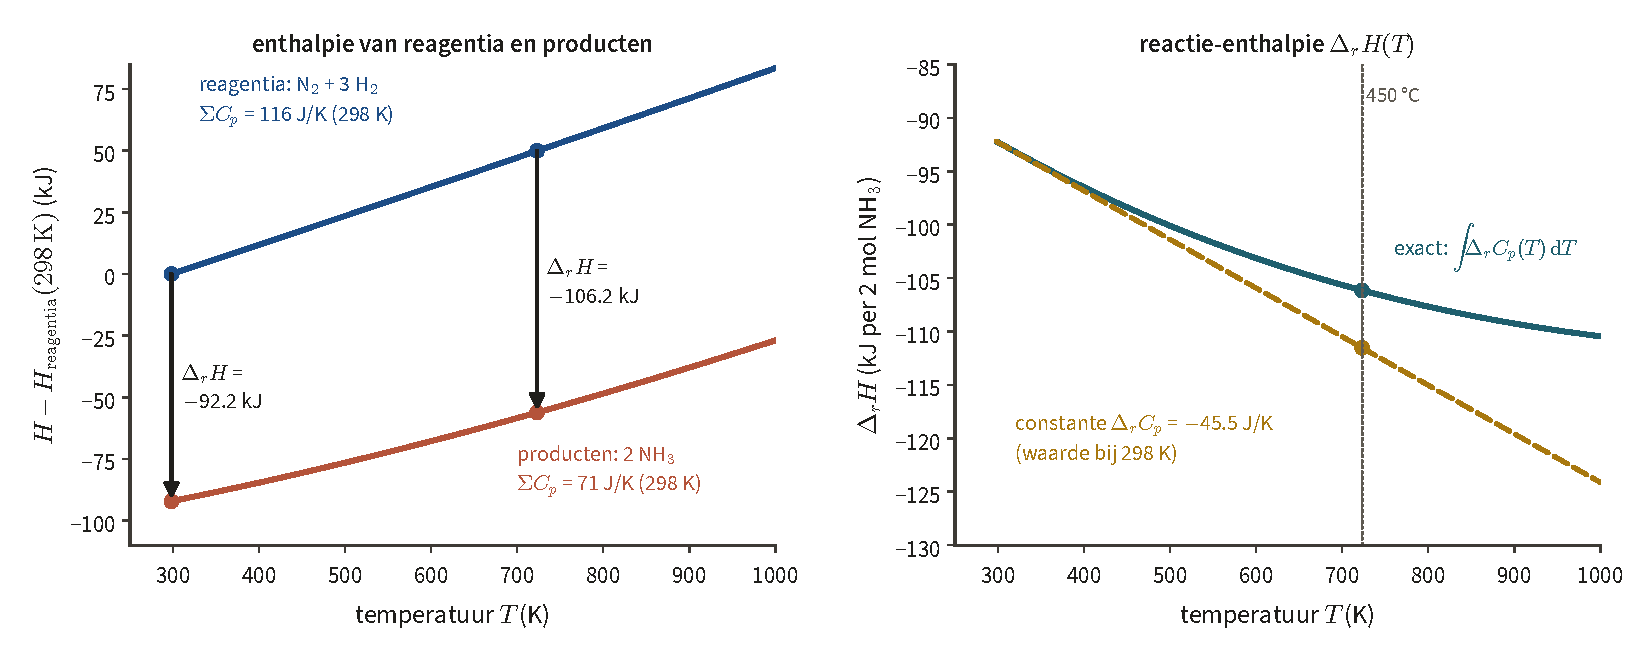
\includegraphics[width=\textwidth]{Figuren/kirchhoff}
    \caption{De wet van Kirchhoff voor de ammoniaksynthese \ce{N2 + 3 H2 -> 2 NH3}. Links: enthalpie van reagentia en producten (ten opzichte van de reagentia bij \SI{298}{\kelvin}); de helling van elke lijn is zijn warmtecapaciteit, de verticale afstand is $\Delta_r H$. Rechts: $\Delta_r H(T)$ met de temperatuurafhankelijke $C_p$ uit tabel~\ref{tab:cp_coeff} en met de constante waarde $\Delta_r C_p(\SI{298}{\kelvin})$.}
    \label{fig:kirchhoff}
\end{figure}

\paragraph{Constante $\Delta_r C_p$.} Over een beperkt temperatuurinterval mag je $\Delta_r C_p^\circ$ constant nemen, en dan wordt de integraal eenvoudig:
\begin{equation}
\Delta_r H^\circ(T) \approx \Delta_r H^\circ(T_0) + \Delta_r C_p^\circ\,(T - T_0).
\label{eq:kirchhoff-constant}
\end{equation}
Dat is een rechte in figuur~\ref{fig:kirchhoff} (rechts). Hoe groter het temperatuurverschil, hoe meer ze afwijkt van de echte kromme, omdat de warmtecapaciteiten zelf met $T$ veranderen (figuur~\ref{fig:cp-temperatuur}).

\begin{voorbeeld}{Vormingsenthalpie van waterdamp bij \SI{100}{\celsius}}
De standaardvormingsenthalpie van waterdamp bij \SI{25}{\celsius} is \SI{-241.82}{\kilo\joule\per\mole}. Hoeveel is ze bij \SI{100}{\celsius}? De vormingsreactie is
\[
\ce{H2(g) + 1/2 O2(g) -> H2O(g)}.
\]
Met $C_{p,\mathrm{m}}^\circ$ bij \SI{298}{\kelvin} (\ce{H2O(g)} 33.58, \ce{H2} 28.82, \ce{O2} \SI{29.36}{\joule\per\mole\per\kelvin}; Atkins \& de Paula):
\[
\Delta_r C_p^\circ = 33.58 - 28.82 - \tfrac12(29.36) = \SI{-9.92}{\joule\per\mole\per\kelvin}.
\]
Over \SI{75}{\kelvin} is $\Delta_r C_p$ zeker constant, dus
\[
\Delta_f H^\circ(\SI{373}{\kelvin}) = -241.82 + (-9.92\times10^{-3})(75) = \SI{-242.56}{\kilo\joule\per\mole}.
\]
Een verschuiving van amper \SI{0.3}{\percent}: over enkele tientallen kelvin mag je de tabelwaarde meestal gewoon gebruiken.
\end{voorbeeld}

\begin{voorbeeld}{Ammoniaksynthese bij \SI{450}{\celsius}}
In het Haber-Boschproces reageert \ce{N2 + 3 H2 -> 2 NH3} bij ongeveer \SI{723}{\kelvin}. Bij \SI{298}{\kelvin} is $\Delta_r H^\circ = 2(\SI{-46.1}{\kilo\joule\per\mole}) = \SI{-92.2}{\kilo\joule}$. Hoeveel warmte moet de koeling van de reactor per 2 mol \ce{NH3} afvoeren bij de procestemperatuur?

\emph{Stap 1: $\Delta_r C_p$ als veelterm.} Met $C_p = a + bT + cT^2$ uit tabel~\ref{tab:cp_coeff} combineer je de co\"effici\"enten zoals de stoffen in de reactie:
\begin{align*}
\Delta a &= 2(24.4) - 28.5 - 3(29.1) = -67.0,\\
\Delta b &= 2(3.86\times10^{-2}) - 3.6\times10^{-4} - 3(-6.1\times10^{-4}) = 7.87\times10^{-2},\\
\Delta c &= 2(-6.40\times10^{-6}) - 4.00\times10^{-6} - 3(1.65\times10^{-6}) = -2.18\times10^{-5}.
\end{align*}
Bij \SI{298}{\kelvin} is $\Delta_r C_p = \SI{-45.5}{\joule\per\kelvin}$, bij \SI{723}{\kelvin} nog maar \SI{-21.5}{\joule\per\kelvin}.

\emph{Stap 2: integreren} van \SI{298}{\kelvin} tot \SI{723}{\kelvin}, term per term zoals bij de opwarming van lucht:
\begin{align*}
\int_{298}^{723} \Delta_r C_p\,\dd T &= \Delta a\,(425) + \frac{\Delta b}{2}(723^2 - 298^2) + \frac{\Delta c}{3}(723^3 - 298^3)\\
&= -28.5 + 17.1 - 2.5 = \SI{-14.0}{\kilo\joule}.
\end{align*}
\emph{Stap 3: optellen.}
\[
\Delta_r H^\circ(\SI{723}{\kelvin}) = -92.2 - 14.0 = \SI{-106.2}{\kilo\joule}.
\]
Bij de procestemperatuur komt dus \SI{15}{\percent} meer warmte vrij dan de tabelwaarde doet vermoeden, en dat moet de koeling aankunnen. Had je $\Delta_r C_p$ constant op zijn waarde bij \SI{298}{\kelvin} gehouden, dan vond je $-92.2 + (-45.5\times10^{-3})(425) = \SI{-111.5}{\kilo\joule}$: de fout van \SI{5}{\kilo\joule} is ruim een derde van de correctie zelf (figuur~\ref{fig:kirchhoff}, rechts). Over honderden kelvin gebruik je dus beter de temperatuurafhankelijke $C_p$.
\end{voorbeeld}


\section{Warmte-effecten van reacties: de adiabatische temperatuur}
\label{sec:warmte-effecten}

Een reactie-enthalpie uit een tabel lijkt een abstract getal. In een reactor wordt ze heel concreet: de vrijgekomen warmte moet ergens heen. Ofwel wordt ze afgevoerd via een koelmantel of warmtewisselaar, ofwel blijft ze in het reactiemengsel en stijgt de temperatuur. Voor de ingenieur is de belangrijkste vraag dan: \emph{hoe warm wordt het mengsel als er niet gekoeld wordt?}

\subsection{De energiebalans over een reactor}

Omdat enthalpie een toestandsfunctie is, mogen we de weg van reagentia naar producten zelf kiezen. De eenvoudigste weg bestaat uit twee stappen:
\begin{enumerate}
\item de reactie laten verlopen bij \SI{298}{\kelvin}: de enthalpie verandert met $\xi\,\Delta_r H^\circ(\SI{298}{\kelvin})$, met $\xi$ het aantal mol omgezet;
\item het productmengsel opwarmen van \SI{298}{\kelvin} tot de eindtemperatuur $T$: de enthalpie verandert met $\sum_i n_i \int_{298}^{T} C_{p,i}\,\dd T$, gesommeerd over alle stoffen die de reactor verlaten (ook inerte stoffen zoals stikstof).
\end{enumerate}
Bij een \emph{adiabatische} reactor ($Q = 0$, geen asarbeid) is de totale enthalpieverandering nul. De eindtemperatuur, de \emph{adiabatische temperatuur} $T_\mathrm{ad}$, volgt dus uit
\begin{equation}
\boxed{\;0 = \xi\,\Delta_r H^\circ(\SI{298}{\kelvin}) + \sum_{i,\,\mathrm{uit}} n_i \int_{298}^{T_\mathrm{ad}} C_{p,i}\,\dd T\;}
\label{eq:adiabatische-temperatuur}
\end{equation}
Bij een exotherme reactie is de eerste term negatief; de tweede term moet die compenseren door een temperatuurstijging. Met een gemiddelde, constante warmtecapaciteit van het productmengsel wordt dit eenvoudig:
\begin{equation}
T_\mathrm{ad} - 298 \approx \frac{\xi\,(-\Delta_r H^\circ)}{\sum_i n_i \overline{C}_{p,i}}.
\label{eq:adiabatische-temperatuur-cp}
\end{equation}
Komt de voeding niet binnen op \SI{298}{\kelvin}, dan voeg je een derde stap toe: de voeding eerst afkoelen (of opwarmen) tot \SI{298}{\kelvin}.

\begin{voorbeeld}{Adiabatische vlamtemperatuur van aardgas}
Methaan verbrandt met de stoichiometrische hoeveelheid lucht (\SI{21}{\percent} \ce{O2}, \SI{79}{\percent} \ce{N2}, dus 3.76 mol \ce{N2} per mol \ce{O2}). Voeding en lucht komen binnen op \SI{25}{\celsius}:
\[
\ce{CH4 + 2 O2 + 7.52 N2 -> CO2 + 2 H2O(g) + 7.52 N2}
\]
Het water verlaat de vlam als damp, dus gebruiken we $\Delta_r H^\circ = \SI{-802.3}{\kilo\joule\per\mole}$ (en niet $-890.3$, dat geldt voor vloeibaar water; het verschil is $2\times\SI{44.0}{\kilo\joule\per\mole}$ verdampingsenthalpie).

Als gemiddelde warmtecapaciteiten tussen \SI{298}{\kelvin} en \SI{2300}{\kelvin} nemen we \ce{CO2}: \SI{54.8}{}, \ce{H2O}: \SI{44.2}{} en \ce{N2}: \SI{33.5}{\joule\per\mole\per\kelvin}. Per mol methaan:
\[
\sum_i n_i\overline{C}_{p,i} = 54.8 + 2(44.2) + 7.52(33.5) = \SI{395}{\joule\per\kelvin}
\]
\[
T_\mathrm{ad} = 298 + \frac{802\,300}{395} = \SI{2330}{\kelvin}\;(\approx\SI{2060}{\celsius}).
\]
Gemeten vlamtemperaturen liggen iets lager, rond \SI{2220}{\kelvin}. Bij zulke hoge temperaturen valt een klein deel van \ce{CO2} en \ce{H2O} terug uiteen in \ce{CO}, \ce{H2} en \ce{O2} (een evenwicht, hoofdstuk~\ref{ch:reagerend}); die ontbinding slorpt warmte op.

Merk op dat bijna twee derde van de warmtecapaciteit van het rookgas afkomstig is van stikstof, dat niet eens deelneemt aan de reactie. Verbranden met zuivere zuurstof geeft daarom veel hogere temperaturen: een snijbrander met acetyleen en zuurstof haalt meer dan \SI{3300}{\kelvin}.
\end{voorbeeld}

\begin{figure}[htb]
    \centering
    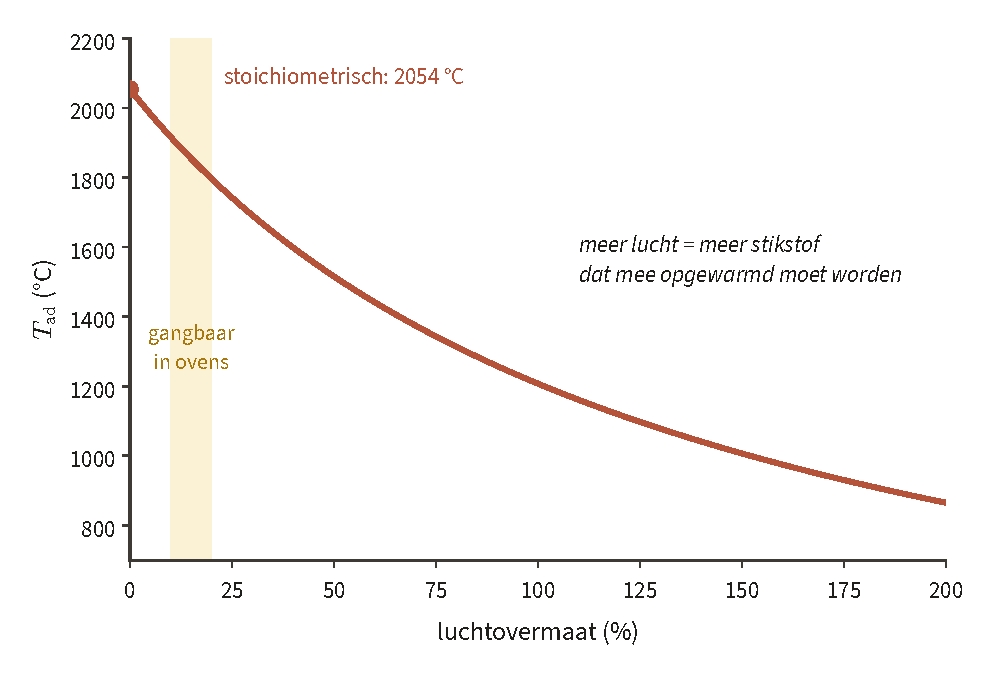
\includegraphics[width=0.7\linewidth]{Figuren/vlamtemperatuur}
    \caption{Adiabatische vlamtemperatuur van methaan als functie van de luchtovermaat, berekend met temperatuurafhankelijke warmtecapaciteiten (NIST). Elke extra kilogram lucht moet mee opgewarmd worden en verlaagt de eindtemperatuur. Ovens werken meestal met 10 tot 20\,\% luchtovermaat: genoeg om volledige verbranding te verzekeren, niet zoveel dat de vlam te sterk afkoelt.}
    \label{fig:vlamtemperatuur}
\end{figure}

\subsection{Adiabatische temperatuurstijging in een vloeistofreactor}

In een vloeistofreactor is het oplosmiddel (vaak water) de grootste warmtebuffer. Per liter reactiemengsel met beginconcentratie $c_{A,0}$ van de reagens en volumieke warmtecapaciteit $\rho c_p$ wordt vergelijking~(\ref{eq:adiabatische-temperatuur-cp}) bij volledige omzetting:
\begin{equation}
\boxed{\Delta T_\mathrm{ad} = \frac{c_{A,0}\,(-\Delta_r H)}{\rho\,c_p}}
\label{eq:delta-T-ad}
\end{equation}
Dit getal is een eerste veiligheidscontrole voor elke exotherme reactie: het is de temperatuurstijging die optreedt als de koeling volledig uitvalt.

\begin{voorbeeld}{Wat als de koeling uitvalt?}
In een batchreactor verloopt een hydrogenering in waterig midden met $c_{A,0} = \SI{2.0}{\mole\per\litre}$ en $\Delta_r H = \SI{-100}{\kilo\joule\per\mole}$. Met $\rho c_p \approx \SI{4.18}{\kilo\joule\per\litre\per\kelvin}$:
\[
\Delta T_\mathrm{ad} = \frac{(2.0)(100)}{4.18} = \SI{48}{\kelvin}.
\]
Start de reactor op \SI{60}{\celsius}, dan kan het mengsel bij uitval van de koeling tot \SI{108}{\celsius} opwarmen: boven het kookpunt van water. De druk in de reactor loopt op, en bovendien versnelt de reactie sterk bij hogere temperatuur. In hoofdstuk~\ref{ch:kinetiek} zien we hoe die combinatie kan leiden tot een \emph{thermal runaway}.

Een vuistregel uit de procesveiligheid: bij $\Delta T_\mathrm{ad}$ kleiner dan ongeveer \SI{50}{\kelvin} is het risico beperkt; bij meer dan \SI{200}{\kelvin} is een grondige veiligheidsstudie nodig.
\end{voorbeeld}

\begin{toepassing}{Tussenkoeling, opnieuw}
Bij de compressor zagen we dat tussenkoeling de eindtemperatuur beperkt. Exotherme gasreactoren werken volgens hetzelfde principe. In een zwavelzuurfabriek wordt \ce{SO2} omgezet tot \ce{SO3} in vier katalysatorbedden na elkaar. In elk bed stijgt de temperatuur adiabatisch; tussen de bedden koelt een warmtewisselaar het gas opnieuw af. De vrijgekomen warmte wordt zo meteen nuttig gebruikt om stoom te maken. Waarom de temperatuur laag moet blijven, ondanks dat de reactie dan trager verloopt, zie je in hoofdstuk~\ref{ch:reagerend}: bij een exotherme reactie daalt de evenwichtsomzetting met de temperatuur.
\end{toepassing}

\section{Faseovergangen en overgangsenthalpie\"en}

Bij smelten, verdampen of sublimeren wordt warmte opgenomen zonder dat de temperatuur verandert (figuur~\ref{fig:opwarmcurve}). De warmte per mol bij constante druk is de \emph{overgangsenthalpie}: $\Delta H_\text{fus}$ (smelten), $\Delta H_\text{vap}$ (verdampen) en $\Delta H_\text{sub} = \Delta H_\text{fus} + \Delta H_\text{vap}$ (sublimeren). Voor water is $\Delta H_\text{fus} = \SI{6.0}{\kilo\joule\per\mole}$ bij \SI{0}{\celsius} en $\Delta H_\text{vap} = \SI{40.7}{\kilo\joule\per\mole}$ bij \SI{100}{\celsius}. De energie gaat naar het verbreken van intermoleculaire bindingen (hoofdstuk~\ref{ch:intermoleculair}).

\begin{figure}[htb]
    \centering
    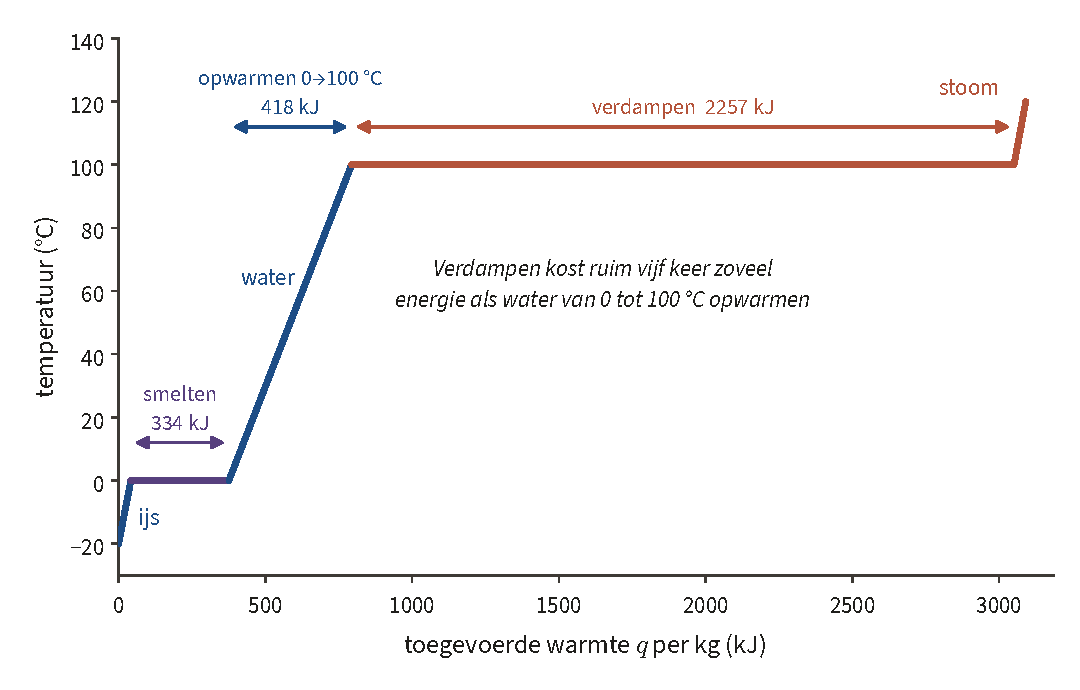
\includegraphics[width=0.7\linewidth]{Figuren/opwarmcurve_water}
    \caption{Temperatuur van \SI{1}{\kilogram} water bij gelijkmatige warmtetoevoer, van ijs bij \SI{-20}{\celsius} tot stoom bij \SI{120}{\celsius}. Tijdens smelten en verdampen blijft de temperatuur constant.}
    \label{fig:opwarmcurve}
\end{figure}

\begin{voorbeeld}{Verdampen van water}
Om \SI{1}{\mole} water op te warmen van \SI{0}{\celsius} tot \SI{100}{\celsius} is $C_p\Delta T = (75.3)(100) = \SI{7.53}{\kilo\joule}$ nodig. Om het daarna te verdampen: \SI{40.7}{\kilo\joule}, 5.4 keer meer. Van de totale \SI{48.2}{\kilo\joule} gaat dus meer dan \SI{80}{\percent} naar de faseovergang. Daarom verbruikt de reboiler van een destillatiekolom zoveel meer energie dan een gewone vloeistofverwarmer.
\end{voorbeeld}

\section{De beperkingen van de eerste hoofdwet}

Een hete kop koffie koelt af tot kamertemperatuur; nooit warmt lauwe koffie spontaan op door warmte uit de kamer te halen. Beide processen respecteren de eerste hoofdwet: energie blijft behouden. De eerste hoofdwet zegt dus niets over de \emph{richting} van een proces. Daarvoor is een tweede grootheid nodig, de entropie. Haar moleculaire oorsprong (hoofdstuk~\ref{ch:kwantum}) en haar gevolgen (hoofdstuk~\ref{ch:spontaniteit}) zijn het onderwerp van de volgende twee hoofdstukken.


\section{Samenvatting en reflectie}

\begin{samenvatting}{Energie en de eerste hoofdwet}
\begin{itemize}
\item Een \emph{systeem} is open (massa en energie), gesloten (enkel energie) of ge\"isoleerd (niets). Toestandsfuncties ($U$, $H$, $p$, $T$, \ldots) hangen enkel af van de toestand; warmte en arbeid hangen af van de weg.
\item De ideale gaswet $pV = nRT$ is een limietwet voor $p \to 0$. De kinetische gastheorie verklaart ze: druk ontstaat door botsingen tegen de wand, en $\tfrac{1}{2}M\langle v^2\rangle = \tfrac{3}{2}RT$. Re\"ele gassen beschrijf je met de compressibiliteitsfactor $Z$ of de vergelijking van Van der Waals.
\item Eerste hoofdwet: $\Delta U = Q + W$. Energie gaat nooit verloren, ze verandert enkel van vorm.
\item Enthalpie $H = U + pV$ is de natuurlijke grootheid voor processen bij constante druk en voor stromende systemen: $\Delta H = Q_p$.
\item Warmtecapaciteit: $\Delta H = \int C_p\,\dd T$. Voor een ideaal gas geldt $C_p - C_V = R$.
\item Reactie-enthalpie\"en volgen uit vormingsenthalpie\"en (wet van Hess) en worden met de wet van Kirchhoff naar andere temperaturen omgerekend.
\item De adiabatische temperatuur volgt uit $0 = \xi\Delta_r H^\circ + \sum n_i\int C_{p,i}\,\dd T$. Ze bepaalt vlamtemperaturen en is de eerste veiligheidscontrole voor exotherme reactoren.
\item Faseovergangen vragen veel energie bij constante temperatuur: verdampen van water kost ruim vijf keer meer dan opwarmen van 0 tot \SI{100}{\celsius}.
\end{itemize}
\end{samenvatting}

\begin{reflectie}{Energie en de eerste hoofdwet}
\begin{enumerate}
\item Waarom is de hoogte van een berg een toestandsfunctie, maar de lengte van het pad naar de top niet? Geef een thermodynamisch equivalent van beide.
\item Een fietsband voelt warm aan na het oppompen. Leg uit met de eerste hoofdwet \'en met het moleculaire beeld van de kinetische gastheorie.
\item Waarom gebruik je voor een warmtewisselaar of een reactor de enthalpie en niet de interne energie?
\item Waarom loopt een heliumballon sneller leeg dan een ballon gevuld met lucht?
\item Een oven verbrandt aardgas met \SI{100}{\percent} luchtovermaat in plaats van \SI{10}{\percent}. Wat gebeurt er met de vlamtemperatuur, en waarom is dat nadelig voor het rendement van de oven?
\item Twee reacties hebben dezelfde $\Delta_r H$, maar de ene loopt in een verdunde oplossing en de andere in een geconcentreerde. Welke is gevaarlijker bij uitval van de koeling?
\item Waarom kan de eerste hoofdwet niet voorspellen of een kop koffie spontaan afkoelt of opwarmt?
\end{enumerate}
\end{reflectie}

\newpage
\section{Oefeningen}

% Oefeningen bij hoofdstuk 1 (wordt ingevoegd achteraan Energie.tex).
% Een oefening:  \begin{oefening} ... \end{oefening}   (boek en website)
% De oplossing:  \begin{oplossing} ... \end{oplossing}       (enkel website, dichtgeklapt)

Neem $R = \SI{8.314}{\joule\per\mole\per\kelvin}$ tenzij anders vermeld.

\begin{oefening}
Een industri\"ele compressor comprimeert \SI{100}{\mole} stikstof (ideaal gas) isotherm bij \SI{300}{\kelvin} van \SI{1}{\bar} naar \SI{50}{\bar}. Bereken
\begin{enumerate}
\item[(a)] de benodigde reversibele arbeid,
\item[(b)] de warmte die aan de omgeving moet worden afgevoerd,
\item[(c)] het volume van het gas voor en na de compressie.
\end{enumerate}
\end{oefening}
\begin{oplossing}
\textbf{Resultaat:} (a) $W = \SI{976}{\kilo\joule}$. (b) $Q = \SI{-976}{\kilo\joule}$. (c) $V_1 = \SI{2.49}{\metre\cubed}$, $V_2 = \SI{0.050}{\metre\cubed}$.

\textbf{(a)} Voor een reversibele isotherme compressie van een ideaal gas geldt $W = nRT\ln(p_2/p_1)$:
\[
W = (100)(8.314)(300)\ln 50 = 9.76\times 10^{5}\,\mathrm{J} \approx 976\,\mathrm{kJ}
\]

\textbf{(b)} Isotherm en ideaal gas: $\Delta U = 0$, dus $Q = -W = -976\,\mathrm{kJ}$. Alle toegevoerde arbeid moet als warmte worden afgevoerd (in de praktijk via tussenkoelers).

\textbf{(c)} $V_1 = nRT/p_1 = (100)(8.314)(300)/(1\times10^5) = 2.49\,\mathrm{m^3}$ en $V_2 = V_1/50 = 0.0499\,\mathrm{m^3} \approx 50\,\mathrm{L}$.
\end{oplossing}

\begin{oefening}
Dezelfde compressor werkt nu adiabatisch ($Q = 0$) en reversibel. De begin temperatuur bedraagt \SI{300}{\kelvin}. Neem $C_{V,m} = \frac{5}{2}R$ voor $\mathrm{N_2}$ (tweatomig ideaal gas).
\begin{enumerate}
\item[(a)] Bereken de eindtemperatuur bij een compressie van \SI{1}{\bar} naar \SI{50}{\bar}.
\item[(b)] Bereken de benodigde arbeid per mol.
\item[(c)] Vergelijk met de isotherme arbeid uit Oefening 1. Verklaar waarom de adiabatische arbeid groter is.
\end{enumerate}
\emph{Hint:} voor een reversibele adiabatische compressie van een ideaal geldt $T_2/T_1 = (p_2/p_1)^{R/C_{p,m}}$.    
\end{oefening}
\begin{oplossing}
\textbf{Resultaat:} (a) $T_2 = \SI{917}{\kelvin}$ (\SI{644}{\celsius}). (b) $W = \SI{12.8}{\kilo\joule\per\mole}$. (c) Isotherm slechts \SI{9.76}{\kilo\joule\per\mole}: de adiabatische compressie vraagt ongeveer 30\,\% meer arbeid.

\textbf{(a)} Met de wet van Mayer is $C_{p,m} = C_{V,m} + R = \frac{7}{2}R$, zodat $R/C_{p,m} = 2/7$:
\[
T_2 = 300 \cdot 50^{2/7} = 300 \cdot 3.06 = 917\,\mathrm{K}
\]

\textbf{(b)} Met $Q = 0$ volgt uit de eerste hoofdwet $W = \Delta U = C_{V,m}(T_2 - T_1)$:
\[
W = \tfrac{5}{2}(8.314)(917-300) = 1.28\times10^{4}\,\mathrm{J/mol} = 12.8\,\mathrm{kJ/mol}
\]

\textbf{(c)} Isotherm: $W/n = RT\ln 50 = 9.76\,\mathrm{kJ/mol}$. Omdat het gas tijdens de adiabatische compressie opwarmt, ligt de druk bij elk volume hoger dan bij de isotherme compressie; de adiabaat ligt in het $p$-$V$-diagram boven de isotherm, en de oppervlakte eronder (de arbeid) is dus groter. Daarom gebruikt men in de industrie meertrapscompressie met tussenkoeling: zo benadert men de goedkopere isotherme compressie, en vermijdt men bovendien eindtemperaturen van meer dan \SI{600}{\celsius} die smering en materialen zouden beschadigen.
\end{oplossing}

\begin{oefening}
Een processtroom van \SI{2.0}{\kilogram\per\second} water wordt in een warmtewisselaar opgewarmd van \SI{25}{\celsius} naar \SI{85}{\celsius}. De warmtecapaciteit van water bedraagt $C_p \approx \SI{4.18}{\kilo\joule\per\kilogram\per\kelvin}$ en mag constant worden verondersteld.
\begin{enumerate}
\item[(a)] Bereken de benodigde warmtestroom (in \si{\kilo\watt}).
\item[(b)] Bereken de verandering van de enthalpie van de waterstroom per seconde.
\item[(c)] Waarom mag de enthalpieverandering hier gelijk worden gesteld aan de uitgewisseld warmte?
\end{enumerate}    
\end{oefening}
\begin{oplossing}
\textbf{Resultaat:} (a) $\dot Q = \SI{502}{\kilo\watt}$. (b) $\Delta\dot H = \SI{502}{\kilo\joule\per\second}$. (c) Constante druk en geen asarbeid, dus $\Delta H = Q_p$.

\textbf{(a)} $\dot Q = \dot m\, C_p\, \Delta T = (2.0)(4.18)(60) = 502\,\mathrm{kW}$.

\textbf{(b)} $\Delta \dot H = \dot Q = 502\,\mathrm{kJ/s}$.

\textbf{(c)} De warmtewisselaar werkt bij (nagenoeg) constante druk, er wordt geen asarbeid verricht en veranderingen in kinetische en potenti\"ele energie zijn verwaarloosbaar. Uit $\mathrm{d}H = \delta Q + V\,\mathrm{d}p$ met $\mathrm{d}p = 0$ volgt dan $\Delta H = Q_p$.
\end{oplossing}

\begin{oefening}
Bereken de standaardreactie-enthalpie van de verbranding van vloeibaar ethanol:
\[
\mathrm{C_2H_5OH(l) + 3\,O_2(g) \rightarrow 2\,CO_2(g) + 3\,H_2O(l)}.
\]
Gegeven zijn de standaardvormingsenthalpie\"en bij \SI{298}{\kelvin}:
\begin{itemize}
\item $\Delta H_f^\circ(\mathrm{C_2H_5OH,l}) = \SI{-277.7}{\kilo\joule\per\mole}$
\item $\Delta H_f^\circ(\mathrm{CO_2,g}) = \SI{-393.5}{\kilo\joule\per\mole}$
\item $\Delta H_f^\circ(\mathrm{H_2O,l}) = \SI{-285.8}{\kilo\joule\per\mole}$
\item $\Delta H_f^\circ(\mathrm{O_2,g}) = 0$
\end{itemize}
Hoeveel warmte komt vrij bij de verbranding van \SI{1}{\kilogram} ethanol?    
\end{oefening}
\begin{oplossing}
\textbf{Resultaat:} $\Delta_r H^\circ = \SI{-1366.7}{\kilo\joule\per\mole}$; per kg ethanol komt \SI{29.7}{\mega\joule} vrij.

Met de wet van Hess:
\[
\Delta_r H^\circ = 2(-393.5) + 3(-285.8) - (-277.7) - 3(0) = -1366.7\,\mathrm{kJ/mol}
\]
Met $M(\mathrm{C_2H_5OH}) = 46.07\,\mathrm{g/mol}$ bevat \SI{1}{\kilogram} ethanol \SI{21.7}{\mole}, zodat er $21.7 \times 1366.7 \approx 2.97\times10^{4}\,\mathrm{kJ} = 29.7\,\mathrm{MJ}$ warmte vrijkomt. Ter vergelijking: benzine levert ongeveer \SI{45}{\mega\joule\per\kilogram}. Een auto op bio-ethanol (E85) verbruikt daarom merkbaar meer liter per 100~km.
\end{oplossing}

\begin{oefening}
De standaardreactie-enthalpie van de ammoniaksynthese
\[
\mathrm{N_2(g) + 3\,H_2(g) \rightarrow 2\,NH_3(g)}
\]
bedraagt $\Delta_r H^\circ(\SI{298}{\kelvin}) = \SI{-92.4}{\kilo\joule\per\mole}$. De molair warmtecapaciteiten (constant verondersteld) zijn:
\begin{itemize}
\item $C_{p,m}(\mathrm{N_2}) = \SI{29.1}{\joule\per\mole\per\kelvin}$
\item $C_{p,m}(\mathrm{H_2}) = \SI{28.8}{\joule\per\mole\per\kelvin}$
\item $C_{p,m}(\mathrm{NH_3}) = \SI{35.1}{\joule\per\mole\per\kelvin}$
\end{itemize}
Bereken de reactie-enthalpie bij \SI{500}{\celsius} (\SI{773}{\kelvin}). Is de reactie bij hoge temperatuur meer of minder exotherm dan bij kamertemperatuur? Verklaar.    
\end{oefening}
\begin{oplossing}
\textbf{Resultaat:} $\Delta_r C_p^\circ = \SI{-45.3}{\joule\per\mole\per\kelvin}$ en $\Delta_r H^\circ(\SI{773}{\kelvin}) = \SI{-113.9}{\kilo\joule\per\mole}$: met deze gegevens wordt de reactie bij hoge temperatuur \emph{meer} exotherm.

\[
\Delta_r C_p^\circ = 2(35.1) - 29.1 - 3(28.8) = -45.3\,\mathrm{J/(mol\cdot K)}
\]
Met de wet van Kirchhoff:
\[
\Delta_r H^\circ(773\,\mathrm{K}) = -92.4 + (-45.3\times10^{-3})(773-298) = -92.4 - 21.5 = -113.9\,\mathrm{kJ/mol}
\]
De reden is dat $\Delta_r C_p^\circ < 0$: de producten (2~mol $\mathrm{NH_3}$) hebben samen een kleinere warmtecapaciteit dan de reagentia (4~mol gas). Bij opwarmen van 298~K naar 773~K neemt de enthalpie van de reagentia dus sterker toe dan die van de producten, waardoor het enthalpieverschil groter wordt. Nauwkeurige tabelwaarden (met temperatuurafhankelijke $C_p$) geven ongeveer $-105$ \`a $-110\,\mathrm{kJ/mol}$: ook daar wordt de reactie meer exotherm. Wat wel waar is: de evenwichtsligging wordt bij hoge temperatuur ongunstiger (hoofdstuk~3), maar dat heeft te maken met $\Delta_r G^\circ$, niet met een kleinere reactiewarmte.
\end{oplossing}

\begin{oefening}
Een stoomketel moet \SI{10}{\mole} water per minuut omzetten van vloeibaar water bij \SI{25}{\celsius} naar droge verzadigde stoom bij \SI{100}{\celsius} en \SI{1}{\bar}. Gebruik de volgende gegevens:
\begin{itemize}
\item $C_{p,m}(\text{water, vloeibaar}) \approx \SI{75.3}{\joule\per\mole\per\kelvin}$
\item $\Delta H_{\text{vap}} \approx \SI{40.7}{\kilo\joule\per\mole}$ bij \SI{100}{\celsius}
\end{itemize}
\begin{enumerate}
\item[(a)] Bereken de totale warmte die per minuut moet worden toegevoerd.
\item[(b)] Splits deze op in de bijdrage van opwarmen en de bijdrage van verdampen.
\item[(c)] Wat is de verhouding van beide bijdragen? Wat leert dit over het energie\"erverbruik van een reboiler versus een gewone vloeistofverwarmer?
\end{enumerate}    
\end{oefening}
\begin{oplossing}
\textbf{Resultaat:} (a) \SI{463}{\kilo\joule} per minuut (\SI{7.7}{\kilo\watt}). (b) Opwarmen \SI{56.5}{\kilo\joule}, verdampen \SI{407}{\kilo\joule}. (c) Verhouding 7.2: 88\,\% van de energie gaat naar de faseovergang.

\textbf{(b)} Opwarmen: $Q_1 = n\,C_{p,m}\,\Delta T = (10)(75.3)(75) = 56.5\,\mathrm{kJ}$. Verdampen: $Q_2 = n\,\Delta H_{\text{vap}} = (10)(40.7) = 407\,\mathrm{kJ}$.

\textbf{(a)} $Q = Q_1 + Q_2 = 463\,\mathrm{kJ}$ per minuut, of een vermogen van $463/60 = 7.7\,\mathrm{kW}$.

\textbf{(c)} $Q_2/Q_1 = 7.2$. Een reboiler, die vloeistof verdampt, verbruikt daardoor veel meer energie dan een verwarmer die dezelfde stroom enkel opwarmt. Dat is ook waarom destillatie een van de meest energie-intensieve operaties in de chemische industrie is, en waarom je thuis veel minder energie verbruikt om water tot het kookpunt te brengen dan om het weg te koken.
\end{oplossing}

\begin{oefening}
Koolstofdioxide bij hoge druk wijkt sterk af van ideaal gedrag. De Van der Waals-constanten voor $\mathrm{CO_2}$ zijn $a = \SI{0.364}{\pascal\metre\tothe{6}\per\mole\tothe{2}}$ en $b = \SI{4.27e-5}{\metre\cubed\per\mole}$.
\begin{enumerate}
\item[(a)] Bereken de druk die de vergelijking van Van der Waals voorspelt voor \SI{1}{\mole} $\mathrm{CO_2}$ bij $T = \SI{300}{\kelvin}$ en $V_m = \SI{0.5}{\litre\per\mole}$.
\item[(b)] Vergelijk met de druk die de ideale gaswet voorspelt onder dezelfde omstandigheden.
\item[(c)] Bereken de compressibiliteitsfactor $Z$ in beide gevallen. Verklaar waarom $Z < 1$.
\end{enumerate}    
\end{oefening}
\begin{oplossing}
\textbf{Resultaat:} (a) $p_{\text{vdW}} = \SI{40.0}{\bar}$. (b) $p_{\text{ideaal}} = \SI{49.9}{\bar}$. (c) $Z_{\text{vdW}} = 0.80$, $Z_{\text{ideaal}} = 1$; de aantrekkingskrachten domineren.

\textbf{(a)} Met $V_m = 5.0\times10^{-4}\,\mathrm{m^3/mol}$:
\[
p = \frac{RT}{V_m - b} - \frac{a}{V_m^2} = \frac{(8.314)(300)}{4.573\times10^{-4}} - \frac{0.364}{2.5\times10^{-7}} = 5.45\times10^{6} - 1.46\times10^{6} = 4.00\times10^{6}\,\mathrm{Pa}
\]

\textbf{(b)} $p_{\text{ideaal}} = RT/V_m = 4.99\times10^{6}\,\mathrm{Pa} \approx 50\,\mathrm{bar}$. De ideale gaswet overschat de druk met ongeveer 25\,\%.

\textbf{(c)} $Z_{\text{vdW}} = pV_m/(RT) = 0.80$. Bij deze matige dichtheid domineert de aantrekkingsterm $a/V_m^2$ de volumecorrectie $b$: de intermoleculaire aantrekking verlaagt de druk op de wand, zodat $Z < 1$.
\end{oplossing}

\begin{oefening}
Je zet een waterkoker van \SI{2200}{\watt} aan met \SI{1.5}{\litre} kraantjeswater van \SI{15}{\celsius}. Neem aan dat 90\,\% van het elektrisch vermogen in het water terechtkomt en dat $C_p = \SI{4.18}{\kilo\joule\per\kilogram\per\kelvin}$.
\begin{enumerate}
\item[(a)] Hoeveel warmte is nodig om het water tot \SI{100}{\celsius} te brengen?
\item[(b)] Hoe lang duurt dat?
\item[(c)] Wat kost het, bij een elektriciteitsprijs van 0.30~euro/kWh?
\item[(d)] Je vergeet de waterkoker en hij schakelt niet af. Hoeveel extra tijd is nodig om de helft van het water weg te koken? Gebruik $\Delta H_{\text{vap}} = \SI{2257}{\kilo\joule\per\kilogram}$.
\end{enumerate}
\end{oefening}
\begin{oplossing}
\textbf{Resultaat:} (a) \SI{533}{\kilo\joule}. (b) Ongeveer 4.5~min. (c) \SI{0.164}{\kilo\watt\hour}, ongeveer 5~eurocent. (d) Nog ongeveer 14~min extra.

\textbf{(a)} $Q = m\,C_p\,\Delta T = (1.5)(4.18)(85) = 533\,\mathrm{kJ}$.

\textbf{(b)} Het nuttig vermogen is $0.9 \times 2200 = 1980\,\mathrm{W}$, dus $t = 533\,000/1980 = 269\,\mathrm{s} \approx 4.5\,\mathrm{min}$.

\textbf{(c)} Elektrische energie $= 533/0.9 = 592\,\mathrm{kJ} = 0.164\,\mathrm{kWh}$, of ongeveer 5~eurocent.

\textbf{(d)} $Q = (0.75)(2257) = 1693\,\mathrm{kJ}$, dus $t = 1\,693\,000/1980 = 855\,\mathrm{s} \approx 14\,\mathrm{min}$. Het verdampen van slechts de helft van het water vraagt ruim drie keer zoveel energie als het volledig opwarmen tot het kookpunt (zie ook Oefening~1.6). Daarom loont het om enkel de hoeveelheid water te koken die je nodig hebt, en om een deksel op de kookpot te leggen.
\end{oplossing}

\begin{oefening}
Met een fietspomp comprimeer je lucht van \SI{1}{\bar} en \SI{20}{\celsius} naar \SI{4}{\bar}. Een pompslag gaat zo snel dat de compressie als adiabatisch en reversibel mag worden beschouwd. Behandel lucht als een tweeatomig ideaal gas ($C_{p,m} = \frac{7}{2}R$).
\begin{enumerate}
\item[(a)] Bereken de temperatuur van de lucht aan het einde van de pompslag.
\item[(b)] Bereken de arbeid per mol lucht.
\item[(c)] In werkelijkheid wordt de pomp onderaan hooguit handwarm. Geef twee redenen waarom de berekende temperatuur een overschatting is.
\end{enumerate}
\end{oefening}
\begin{oplossing}
\textbf{Resultaat:} (a) $T_2 = \SI{435}{\kelvin}$ (\SI{162}{\celsius}). (b) $W = \SI{2.96}{\kilo\joule\per\mole}$. (c) Warmteopname door de metalen cilinder en menging met koudere lucht in de band.

\textbf{(a)} $T_2 = T_1 (p_2/p_1)^{R/C_{p,m}} = 293 \cdot 4^{2/7} = 293 \cdot 1.486 = 435\,\mathrm{K} \approx 162\,^\circ\mathrm{C}$.

\textbf{(b)} $W = \Delta U = C_{V,m}\Delta T = \tfrac{5}{2}(8.314)(435-293) = 2.96\,\mathrm{kJ/mol}$.

\textbf{(c)} (1) De metalen cilinder heeft een veel grotere warmtecapaciteit dan de kleine hoeveelheid lucht en neemt de warmte op; elke slag warmt de pomp maar een klein beetje op. (2) De gecomprimeerde lucht stroomt meteen de band in, waar ze mengt met koudere lucht en warmte afgeeft. De compressie is dus niet volledig adiabatisch. Hetzelfde effect zie je bij een dieselmotor, waar de hoge compressietemperatuur juist gebruikt wordt om de brandstof zonder bougie te ontsteken.
\end{oplossing}

\begin{oefening}
In een warmterecuperatiesysteem wordt $\mathrm{CO_2}$ uit rookgassen afgekoeld van \SI{800}{\kelvin} naar \SI{300}{\kelvin}. Gebruik de correlatie $C_p = a + bT + cT^2$ met de co\"effici\"enten uit de tabel in hoofdstuk~1: $a = 22.3$, $b = 5.98\times10^{-2}$, $c = -3.50\times10^{-5}$ (SI-eenheden).
\begin{enumerate}
\item[(a)] Bereken hoeveel warmte per mol $\mathrm{CO_2}$ gerecupereerd kan worden.
\item[(b)] Herhaal de berekening met een constante $C_p$, gelijk aan de waarde bij \SI{300}{\kelvin}.
\item[(c)] Hoe groot is de fout? Wanneer mag je $C_p$ constant veronderstellen?
\end{enumerate}
\end{oefening}
\begin{oplossing}
\textbf{Resultaat:} (a) \SI{21.9}{\kilo\joule\per\mole}. (b) \SI{18.5}{\kilo\joule\per\mole} met $C_p(\SI{300}{\kelvin}) = \SI{37.1}{\joule\per\mole\per\kelvin}$. (c) Een onderschatting van ongeveer 15\,\%.

\textbf{(a)}
\[
\Delta H = a(T_2-T_1) + \frac{b}{2}(T_2^2-T_1^2) + \frac{c}{3}(T_2^3-T_1^3)
\]
Van 300~K naar 800~K: $11\,150 + 16\,445 - 5\,658 = 21\,937\,\mathrm{J/mol}$. Bij afkoeling kan dus $21.9\,\mathrm{kJ/mol}$ gerecupereerd worden.

\textbf{(b)} $C_p(300\,\mathrm{K}) = 22.3 + 17.94 - 3.15 = 37.1\,\mathrm{J/(mol\cdot K)}$, zodat $\Delta H \approx (37.1)(500) = 18.5\,\mathrm{kJ/mol}$.

\textbf{(c)} $\mathrm{CO_2}$ is een lineair drieatomig molecule met buigvibraties die bij hogere temperatuur geactiveerd worden (hoofdstuk~2), waardoor $C_p$ sterk stijgt. Een constante $C_p$ is enkel aanvaardbaar voor kleine temperatuurverschillen, of voor eenvoudige gassen zoals $\mathrm{N_2}$ en edelgassen. Voor het ontwerp van een warmtewisselaar zou deze fout leiden tot een onderdimensionering.
\end{oplossing}

\begin{oefening}
De verbrandingswarmte van een brandstof wordt gemeten in een bomcalorimeter: een gesloten stalen vat met constant volume. Voor methaan,
\[
\mathrm{CH_4(g) + 2\,O_2(g) \rightarrow CO_2(g) + 2\,H_2O(l)},
\]
geldt $\Delta_r H^\circ = \SI{-890.3}{\kilo\joule\per\mole}$ bij \SI{298}{\kelvin}.
\begin{enumerate}
\item[(a)] Meet de bomcalorimeter $\Delta U$ of $\Delta H$? Verklaar.
\item[(b)] Bereken $\Delta_r U^\circ$. Behandel de gassen als ideaal en verwaarloos het volume van vloeibaar water.
\item[(c)] Is het verschil belangrijk voor de dimensionering van een cv-ketel?
\end{enumerate}
\end{oefening}
\begin{oplossing}
\textbf{Resultaat:} (a) $\Delta U$ (constant volume). (b) $\Delta_r U^\circ = \SI{-885.3}{\kilo\joule\per\mole}$. (c) Verschil van slechts 0.6\,\%: verwaarloosbaar voor een cv-ketel.

\textbf{(a)} Bij constant volume wordt geen volumearbeid verricht ($\delta W = -p\,\mathrm{d}V = 0$), zodat $\Delta U = Q_V$.

\textbf{(b)} Uit $H = U + pV$ volgt voor een gasreactie $\Delta_r H = \Delta_r U + \Delta n_{\text{gas}} RT$. Hier is $\Delta n_{\text{gas}} = 1 - 3 = -2$:
\[
\Delta_r U^\circ = \Delta_r H^\circ - \Delta n_{\text{gas}}RT = -890.3 + 2(8.314\times10^{-3})(298) = -885.3\,\mathrm{kJ/mol}
\]

\textbf{(c)} Een cv-ketel werkt bij constante druk, dus de juiste grootheid is $\Delta H$, maar voor het ontwerp is het verschil verwaarloosbaar. Het principe is wel belangrijk: bij reacties met een grote verandering van het aantal mol gas, of bij hoge temperatuur, wordt het verschil groter.
\end{oplossing}

\begin{oefening}
\SI{1}{\mole} lucht (ideaal gas) expandeert isotherm bij \SI{300}{\kelvin} van \SI{10}{\bar} naar \SI{1}{\bar}.
\begin{enumerate}
\item[(a)] Bereken de arbeid voor een reversibele expansie.
\item[(b)] Bereken de arbeid wanneer het gas in \'e\'en keer expandeert tegen een constante uitwendige druk van \SI{1}{\bar}, bijvoorbeeld wanneer je het ventiel van een fles opendraait.
\item[(c)] Bereken in beide gevallen $\Delta U$ en $Q$. Welke grootheden hangen af van de weg, welke niet?
\end{enumerate}
\end{oefening}
\begin{oplossing}
\textbf{Resultaat:} (a) $W_{\text{rev}} = \SI{-5.74}{\kilo\joule}$. (b) $W_{\text{irr}} = \SI{-2.24}{\kilo\joule}$. (c) $\Delta U = 0$ in beide gevallen; $Q_{\text{rev}} = \SI{+5.74}{\kilo\joule}$ en $Q_{\text{irr}} = \SI{+2.24}{\kilo\joule}$. $W$ en $Q$ hangen af van de weg, $\Delta U$ niet.

\textbf{(a)} $W_{\text{rev}} = -nRT\ln(p_1/p_2) = -(8.314)(300)\ln 10 = -5.74\,\mathrm{kJ}$.

\textbf{(b)} $W_{\text{irr}} = -p_{\text{ext}}(V_2 - V_1) = -p_{\text{ext}}\left(\frac{RT}{p_2} - \frac{RT}{p_1}\right) = -RT(1 - 0.1) = -2.24\,\mathrm{kJ}$.

\textbf{(c)} In beide gevallen is $\Delta U = 0$ (isotherm, ideaal gas), dus $Q = -W$. $\Delta U$ is een toestandsfunctie en hangt enkel af van begin- en eindtoestand; $W$ en $Q$ zijn padfuncties. De reversibele weg levert de maximale arbeid. Bij een ventiel dat je gewoon opendraait gaat het grootste deel van die arbeidscapaciteit verloren; een turbine of expander kan een deel ervan w\'el benutten, wat in de industrie toegepast wordt bij het ontspannen van aardgas onder hoge druk.
\end{oplossing}

\begin{oefening}
Je wilt een blikje frisdrank van \SI{330}{\milli\litre} (behandel als water) afkoelen van \SI{25}{\celsius} naar \SI{5}{\celsius} door er ijsblokjes van \SI{0}{\celsius} in te doen. Gebruik $\Delta H_{\text{fus}} = \SI{6.0}{\kilo\joule\per\mole}$ en $C_p = \SI{4.18}{\joule\per\gram\per\kelvin}$. Verwaarloos warmte-uitwisseling met de omgeving.
\begin{enumerate}
\item[(a)] Hoeveel ijs is nodig?
\item[(b)] Hoeveel ijs zou nodig zijn als je in plaats van ijs koud water van \SI{0}{\celsius} gebruikt? Wat besluit je?
\end{enumerate}
\end{oefening}
\begin{oplossing}
\textbf{Resultaat:} (a) \SI{78}{\gram} ijs. (b) \SI{1.3}{\kilogram} koud water: ijs is dankzij de smeltwarmte ongeveer zeventien keer effectiever.

\textbf{(a)} De drank moet $Q = (330)(4.18)(20) = 27.6\,\mathrm{kJ}$ afgeven. De smeltenthalpie per gram bedraagt $6000/18.02 = 333\,\mathrm{J/g}$. Elke gram ijs smelt en het smeltwater warmt nog op van 0 naar \SI{5}{\celsius}, dus neemt $333 + (4.18)(5) = 354\,\mathrm{J/g}$ op. De benodigde massa is $27\,600/354 = 78\,\mathrm{g}$ ijs, ongeveer drie \`a vier ijsblokjes.

\textbf{(b)} Water van \SI{0}{\celsius} dat opwarmt tot \SI{5}{\celsius} neemt slechts $(4.18)(5) = 21\,\mathrm{J/g}$ op: je zou $27\,600/21 = 1.3\,\mathrm{kg}$ nodig hebben, en het blikje loopt over. Dat is hetzelfde principe als bij koelelementen in een koelbox en bij latente-warmteopslag (\emph{phase change materials}) in gebouwen.
\end{oplossing}

\begin{oefening}
Een CNG-wagen heeft een tank van \SI{50}{\litre} waarin \SI{8.0}{\kilogram} methaan zit bij \SI{25}{\celsius}. Voor methaan geldt $T_c = \SI{190.6}{\kelvin}$ en $p_c = \SI{46.0}{\bar}$.
\begin{enumerate}
\item[(a)] Bereken de Van der Waals-parameters $a$ en $b$ van methaan.
\item[(b)] Bereken de druk in de tank met de ideale gaswet en met de vergelijking van Van der Waals.
\item[(c)] Bereken $Z$. Is het voor de tankontwerper gunstig of ongunstig dat methaan niet ideaal is?
\end{enumerate}
\end{oefening}
\begin{oplossing}
\textbf{Resultaat:} (a) $a = 0.230\,\mathrm{Pa\,m^6/mol^2}$, $b = 4.31\times10^{-5}\,\mathrm{m^3/mol}$. (b) Ideaal \SI{247}{\bar}, Van der Waals \SI{204}{\bar}. (c) $Z = 0.83$: gunstig, er past ongeveer 20\,\% meer gas in de tank.

\textbf{(a)}
\[
a = \frac{27R^2T_c^2}{64p_c} = 0.230\,\mathrm{Pa\,m^6/mol^2}, \qquad b = \frac{RT_c}{8p_c} = 4.31\times10^{-5}\,\mathrm{m^3/mol}
\]

\textbf{(b)} $n = 8000/16.04 = 499\,\mathrm{mol}$, dus $V_m = 0.050/499 = 1.00\times10^{-4}\,\mathrm{m^3/mol}$. Ideaal: $p = RT/V_m = 247\,\mathrm{bar}$. Van der Waals: $p = \dfrac{RT}{V_m-b} - \dfrac{a}{V_m^2} = 433.5 - 229.2 = 204\,\mathrm{bar}$.

\textbf{(c)} $Z = pV_m/(RT) = 0.83$. De aantrekking tussen de methaanmoleculen verlaagt de druk: bij een gegeven maximale werkdruk (typisch 200~bar) past er dus ongeveer 20\,\% meer gas in de tank dan de ideale gaswet voorspelt. Een ontwerper die met de ideale gaswet rekent, zou de actieradius van de wagen onderschatten.
\end{oplossing}

\begin{oefening}
Wie een hand boven een kokende waterkoker houdt, verbrandt zich sneller dan wie een paar druppels kokend water op de hand krijgt. Vergelijk \SI{10}{\gram} stoom van \SI{100}{\celsius} met \SI{10}{\gram} vloeibaar water van \SI{100}{\celsius}. Beide komen op de huid terecht en koelen af tot lichaamstemperatuur (\SI{37}{\celsius}). Gebruik $\Delta H_{\text{vap}} = \SI{2257}{\kilo\joule\per\kilogram}$ bij \SI{100}{\celsius} en $C_p = \SI{4.18}{\joule\per\gram\per\kelvin}$ voor vloeibaar water.
\begin{enumerate}
\item[(a)] Hoeveel warmte geeft de stoom af aan de huid? En het kokende water?
\item[(b)] Stel dat die warmte volledig terechtkomt in \SI{50}{\gram} huidweefsel met $C_p \approx \SI{3.5}{\joule\per\gram\per\kelvin}$. Hoeveel zou de temperatuur van dat weefsel stijgen in beide gevallen? Wat besluit je?
\item[(c)] Een stoomoven gaart groenten sneller dan een heteluchtoven op dezelfde temperatuur. Verklaar met hetzelfde principe.
\end{enumerate}
\end{oefening}
\begin{oplossing}
\textbf{Resultaat:} (a) Stoom \SI{25.2}{\kilo\joule}, kokend water \SI{2.6}{\kilo\joule}: stoom levert bijna tien keer meer warmte. (b) Theoretisch \SI{+144}{\kelvin} tegenover \SI{+15}{\kelvin}. (c) De condensatiewarmte komt vrij precies op het oppervlak van het voedsel.

\textbf{(a)} De stoom condenseert eerst bij \SI{100}{\celsius} en daarna koelt het condensaat af tot \SI{37}{\celsius}:
\[
Q_{\text{stoom}} = m\,\Delta H_{\text{vap}} + m\,C_p\,\Delta T = (0.010)(2257) + (10)(4.18)(63)\times10^{-3} = 22.6 + 2.6 = 25.2\,\mathrm{kJ}
\]
Het kokende water levert enkel het tweede deel: $Q_{\text{water}} = 2.6\,\mathrm{kJ}$. De verhouding is ongeveer 9.6.

\textbf{(b)} $\Delta T = Q/(m\,C_p)$: voor stoom $25\,200/(50 \times 3.5) = 144\,\mathrm{K}$, voor water $2630/(50\times3.5) = 15\,\mathrm{K}$. In werkelijkheid voert het bloed een deel van de warmte af, maar de conclusie blijft: bijna 90\,\% van de schade door stoom komt van de condensatie-enthalpie, niet van de temperatuur van \SI{100}{\celsius} zelf. Condensatie is exotherm: wat bij verdampen aan energie werd opgenomen, komt bij condenseren weer vrij.

\textbf{(c)} In een stoomoven condenseert de stoom op het koudere voedsel en geeft daar per kilogram \SI{2257}{\kilo\joule} af. Hete droge lucht kan per kilogram en per kelvin maar ongeveer \SI{1}{\kilo\joule} afgeven en moet dus veel meer warmte via geleiding aanvoeren. Hetzelfde principe gebruikt de industrie in stoomverwarmde warmtewisselaars: verzadigde stoom levert veel warmte bij een constante, goed regelbare temperatuur.
\end{oplossing}

\begin{oefening}
Een druivensuikertablet bevat \SI{3.0}{\gram} glucose ($M = \SI{180.16}{\gram\per\mole}$). De standaardverbrandingsenthalpie van glucose bedraagt $\Delta_c H^\circ = \SI{-2808}{\kilo\joule\per\mole}$. Een persoon van \SI{70}{\kilogram} loopt de trap op; een verdieping is \SI{3.0}{\metre} hoog.
\begin{enumerate}
\item[(a)] Hoeveel warmte zou vrijkomen bij de volledige verbranding van het tablet?
\item[(b)] Hoeveel arbeid kost het om \'e\'en verdieping te stijgen?
\item[(c)] De spieren zetten ongeveer 25\,\% van de chemische energie om in mechanische arbeid. Hoeveel verdiepingen kan de persoon met \'e\'en tablet stijgen?
\item[(d)] De overige energie komt vrij als warmte. Hoeveel zweet moet verdampen om die warmte af te voeren? Neem $\Delta H_{\text{vap}} \approx \SI{2.43}{\kilo\joule\per\gram}$ bij huidtemperatuur.
\end{enumerate}
\end{oefening}
\begin{oplossing}
\textbf{Resultaat:} (a) \SI{46.8}{\kilo\joule}. (b) \SI{2.06}{\kilo\joule} per verdieping. (c) \SI{11.7}{\kilo\joule} arbeid, goed voor \SI{17}{\metre}, of ongeveer vijf \`a zes verdiepingen. (d) Ongeveer \SI{14}{\gram} zweet.

\textbf{(a)} $n = 3.0/180.16 = 0.0167\,\mathrm{mol}$, zodat $|Q| = (0.0167)(2808) = 46.8\,\mathrm{kJ}$.

\textbf{(b)} De arbeid tegen de zwaartekracht is $W = mgh = (70)(9.81)(3.0) = 2.06\,\mathrm{kJ}$.

\textbf{(c)} Nuttige arbeid: $0.25 \times 46.8 = 11.7\,\mathrm{kJ}$. De hoogte is $h = 11\,700/(70 \times 9.81) = 17\,\mathrm{m}$, ongeveer vijf \`a zes verdiepingen.

\textbf{(d)} De overige $0.75 \times 46.8 = 35.1\,\mathrm{kJ}$ is warmte. Om die af te voeren via verdamping is $35.1/2.43 = 14\,\mathrm{g}$ water nodig. De eerste hoofdwet geldt dus ook voor het lichaam: de energie uit voeding verdwijnt niet, maar gaat voor het grootste deel als warmte naar de omgeving. Daarom krijg je het warm bij inspanning, en daarom zweet je.
\end{oplossing}

\begin{oefening}
\begin{enumerate}
\item[(a)] Bereken $v_\mathrm{rms}$ van zuurstof, waterstof en helium bij \SI{20}{\celsius}.
\item[(b)] Waterstof en helium zijn bijna afwezig in de aardatmosfeer, terwijl ze in het heelal het meest voorkomen. Geef een verklaring op basis van (a). De ontsnappingssnelheid van de aarde is \SI{11.2}{\kilo\metre\per\second}; in de bovenste lagen van de atmosfeer loopt de temperatuur op tot meer dan \SI{1000}{\kelvin}.
\item[(c)] Een ballon gevuld met lucht verliest per dag \SI{2}{\percent} van zijn gas door de microporiën van het rubber. Schat hoeveel procent een identieke heliumballon per dag verliest.
\end{enumerate}
\end{oefening}
\begin{oplossing}
\textbf{Resultaat:} (a) \ce{O2}: \SI{478}{\metre\per\second}, \ce{H2}: \SI{1904}{\metre\per\second}, \ce{He}: \SI{1352}{\metre\per\second}. (b) Lichte gassen hebben een snelheidsverdeling met een staart tot boven de ontsnappingssnelheid. (c) Ongeveer \SI{5}{\percent} per dag.

\textbf{(a)} $v_\mathrm{rms} = \sqrt{3RT/M}$ met $T = \SI{293.15}{\kelvin}$:
\[
\ce{O2}: \sqrt{\frac{3(8.314)(293.15)}{0.032}} = 478\,\mathrm{m/s},\qquad
\ce{H2}\ (M = 0.002016): 1904\,\mathrm{m/s},\qquad
\ce{He}\ (M = 0.004003): 1352\,\mathrm{m/s}.
\]

\textbf{(b)} Bij \SI{1000}{\kelvin} is $v_\mathrm{rms}$ van \ce{H2} ongeveer \SI{3.5}{\kilo\metre\per\second}. Dat is nog altijd lager dan \SI{11.2}{\kilo\metre\per\second}, maar $v_\mathrm{rms}$ is een gemiddelde: een kleine fractie van de moleculen is veel sneller (de Maxwell--Boltzmannverdeling, hoofdstuk~\ref{ch:kinetiek}). Over miljarden jaren ontsnappen zo de lichte moleculen uit de bovenste atmosfeer. Voor \ce{O2} en \ce{N2} is die fractie verwaarloosbaar klein.

\textbf{(c)} Volgens de wet van Graham is de effusiesnelheid evenredig met $1/\sqrt{M}$: $\sqrt{28.96/4.003} = 2.69$. De heliumballon verliest dus ongeveer $2.69 \times 2 \approx 5\,\%$ per dag. (In werkelijkheid speelt ook oplossen in en diffunderen door het rubber mee, maar de trend klopt.)
\end{oplossing}

\begin{oefening}
In een batchreactor van \SI{5.0}{\cubic\metre} verloopt een exotherme reactie in waterig midden: $c_{A,0} = \SI{1.5}{\mole\per\litre}$, $\Delta_r H = \SI{-120}{\kilo\joule\per\mole}$, $\rho c_p = \SI{4.0}{\kilo\joule\per\litre\per\kelvin}$. De reactor start bij \SI{70}{\celsius} en de reactie is na \SI{2}{\hour} volledig afgelopen.
\begin{enumerate}
\item[(a)] Bereken de adiabatische temperatuurstijging. Tot welke temperatuur kan het mengsel opwarmen als de koeling uitvalt?
\item[(b)] Welk gemiddeld koelvermogen (in \si{\kilo\watt}) is nodig om de temperatuur constant te houden?
\item[(c)] Om de productie te verhogen wil men de beginconcentratie verdubbelen. Wat is het gevolg voor de veiligheid? Stel een alternatieve werkwijze voor die dezelfde hoeveelheid product oplevert met minder risico.
\end{enumerate}
\end{oefening}
\begin{oplossing}
\textbf{Resultaat:} (a) $\Delta T_\mathrm{ad} = \SI{45}{\kelvin}$, eindtemperatuur \SI{115}{\celsius}. (b) \SI{125}{\kilo\watt}. (c) $\Delta T_\mathrm{ad} = \SI{90}{\kelvin}$, tot \SI{160}{\celsius}; beter een semibatchreactor waarin reagens A geleidelijk wordt toegevoegd.

\textbf{(a)} $\Delta T_\mathrm{ad} = c_{A,0}(-\Delta_r H)/(\rho c_p) = (1.5)(120)/4.0 = 45\,\mathrm{K}$. Het mengsel kan opwarmen tot $70 + 45 = 115\,{}^\circ\mathrm{C}$, boven het kookpunt van water: de druk in de reactor stijgt.

\textbf{(b)} Totale warmte: $(5000\,\mathrm{L})(1.5\,\mathrm{mol/L})(120\,\mathrm{kJ/mol}) = 9.0\times10^5\,\mathrm{kJ}$. Over \SI{7200}{\second} is dat gemiddeld $125\,\mathrm{kW}$. In het begin, wanneer de concentratie het hoogst is, ligt het vermogen hoger dan dit gemiddelde.

\textbf{(c)} De adiabatische temperatuurstijging verdubbelt tot \SI{90}{\kelvin}: het mengsel kan tot \SI{160}{\celsius} oplopen. Omdat de reactiesnelheid sterk stijgt met de temperatuur, kan de reactie dan op hol slaan. Een veiliger alternatief is een \emph{semibatch}werkwijze: je start met het oplosmiddel en de tweede reagens, en doseert A geleidelijk. Er is dan op elk moment maar weinig niet-gereageerde A aanwezig, zodat bij uitval van de koeling de temperatuur slechts weinig stijgt; je stopt dan gewoon de toevoer.
\end{oplossing}

\begin{oefening}
Een industri\"ele oven verbrandt methaan met \SI{20}{\percent} luchtovermaat. Brandstof en lucht komen binnen op \SI{25}{\celsius}. Gebruik $\Delta_c H^\circ = \SI{-802.3}{\kilo\joule\per\mole}$ (water als damp) en de gemiddelde warmtecapaciteiten tussen \SI{298}{\kelvin} en \SI{2100}{\kelvin}: \ce{CO2} \SI{54.1}{}, \ce{H2O} \SI{43.3}{}, \ce{O2} \SI{34.9}{} en \ce{N2} \SI{33.2}{\joule\per\mole\per\kelvin}.
\begin{enumerate}
\item[(a)] Stel de reactievergelijking op, inclusief de overtollige zuurstof en de stikstof.
\item[(b)] Bereken de adiabatische vlamtemperatuur.
\item[(c)] Vergelijk met de stoichiometrische verbranding (\SI{2330}{\kelvin}, zie het voorbeeld in de tekst). Waarom gebruikt men toch luchtovermaat?
\end{enumerate}
\end{oefening}
\begin{oplossing}
\textbf{Resultaat:} (a) $\ce{CH4 + 2.4 O2 + 9.02 N2 -> CO2 + 2 H2O + 0.4 O2 + 9.02 N2}$. (b) $T_\mathrm{ad} \approx \SI{2065}{\kelvin}$ (\SI{1790}{\celsius}). (c) Ongeveer \SI{265}{\kelvin} lager, maar de verbranding is volledig.

\textbf{(a)} Stoichiometrisch is 2 mol \ce{O2} nodig; met 20\,\% overmaat wordt dat 2.4 mol \ce{O2} en $2.4 \times 3.76 = 9.02$ mol \ce{N2}. Er blijft 0.4 mol \ce{O2} over.

\textbf{(b)}
\[
\sum n_i \overline{C}_{p,i} = 54.1 + 2(43.3) + 0.4(34.9) + 9.02(33.2) = 454\,\mathrm{J/K}
\]
\[
T_\mathrm{ad} = 298 + \frac{802\,300}{454} = 2065\,\mathrm{K}.
\]
Een berekening met temperatuurafhankelijke $C_p$ geeft \SI{2070}{\kelvin} (zie figuur~\ref{fig:vlamtemperatuur}).

\textbf{(c)} De extra lucht moet mee opgewarmd worden, zodat de vlam ongeveer \SI{265}{\kelvin} koeler is. Toch is een kleine overmaat nodig: brandstof en lucht mengen nooit perfect, en zonder overmaat ontstaat \ce{CO} (giftig) en roet, en gaat brandstof verloren. Te veel overmaat is evenmin goed: de warme rookgassen voeren dan veel energie mee naar de schoorsteen, en het rendement van de oven daalt.
\end{oplossing}

\begin{oefening}
Waterstof verbrandt stoichiometrisch met lucht: $\ce{H2 + 0.5 O2 + 1.88 N2 -> H2O(g) + 1.88 N2}$, met $\Delta_r H^\circ = \SI{-241.8}{\kilo\joule\per\mole}$. Tussen \SI{300}{\kelvin} en \SI{2500}{\kelvin} geldt in goede benadering $C_p = a + bT$ met
\begin{center}
\begin{tabular}{lcc}
 & $a$ (\si{\joule\per\mole\per\kelvin}) & $b$ (\si{\joule\per\mole\per\kelvin\squared}) \\ \hline
\ce{H2O(g)} & 31.1 & $9.92\times10^{-3}$ \\
\ce{N2} & 28.6 & $3.70\times10^{-3}$ \\
\end{tabular}
\end{center}
\begin{enumerate}
\item[(a)] Stel de energiebalans op voor de adiabatische vlam. Schrijf ze als een vergelijking in $T_\mathrm{ad}$.
\item[(b)] Los de vergelijking op in Excel (bv.\ met \emph{Doelzoeken}) of analytisch.
\item[(c)] Herhaal de berekening met een constante $C_p$, gelijk aan de waarde bij \SI{298}{\kelvin}. Hoe groot is de fout?
\item[(d)] Pas je rekenblad aan voor een luchtovermaat van \SI{50}{\percent}. Neem voor \ce{O2}: $a = 29.9$ en $b = 4.2\times10^{-3}$.
\end{enumerate}
\end{oefening}
\begin{oplossing}
\textbf{Resultaat:} (a) $84.87\,(T-298) + 8.44\times10^{-3}\,(T^2-298^2) = 241\,800$. (b) $T_\mathrm{ad} = \SI{2523}{\kelvin}$. (c) \SI{2988}{\kelvin}, een overschatting met ongeveer \SI{465}{\kelvin}. (d) Ongeveer \SI{1980}{\kelvin}.

\textbf{(a)} Voor het productmengsel geldt $\sum n_i a_i = 31.1 + 1.88(28.6) = 84.87$ en $\sum n_i b_i = 9.92\times10^{-3} + 1.88(3.70\times10^{-3}) = 16.88\times10^{-3}$. Integreren van $C_p$ van \SI{298}{\kelvin} tot $T$ geeft
\[
84.87\,(T - 298.15) + \tfrac{1}{2}(16.88\times10^{-3})(T^2 - 298.15^2) = 241\,800.
\]

\textbf{(b)} Dit is een vierkantsvergelijking in $T$: $8.44\times10^{-3}\,T^2 + 84.87\,T - 267\,850 = 0$, met als positieve wortel $T_\mathrm{ad} = 2523\,\mathrm{K}$. In Excel zet je $T$ in een cel, de linkerzijde min $241\,800$ in een tweede cel, en laat je Doelzoeken die tweede cel op nul brengen. (Met de volledige NIST-gegevens vindt men \SI{2525}{\kelvin}; de lineaire benadering is dus uitstekend.)

\textbf{(c)} Bij \SI{298}{\kelvin}: $C_p(\ce{H2O}) = 34.1$ en $C_p(\ce{N2}) = 29.7\,\mathrm{J/(mol\,K)}$, samen $34.1 + 1.88(29.7) = 89.9\,\mathrm{J/K}$. Dan is $T_\mathrm{ad} = 298 + 241\,800/89.9 = 2988\,\mathrm{K}$: bijna \SI{500}{\kelvin} te hoog. Bij hoge temperatuur worden de vibraties van de moleculen actief (hoofdstuk~\ref{ch:kwantum}), zodat $C_p$ sterk stijgt. Voor grote temperatuursprongen mag je $C_p$ dus niet constant nemen.

\textbf{(d)} Er komt 0.25 mol \ce{O2} en $0.75 \times 3.76 = 2.82$ mol \ce{N2} in de rookgassen: $\sum n_i a_i = 31.1 + 2.82(28.6) + 0.25(29.9) = 119.2$ en $\sum n_i b_i = 9.92\times10^{-3} + 2.82(3.70\times10^{-3}) + 0.25(4.2\times10^{-3}) = 21.40\times10^{-3}$. Doelzoeken geeft $T_\mathrm{ad} \approx 1980\,\mathrm{K}$, ruim \SI{500}{\kelvin} lager dan stoichiometrisch.
\end{oplossing}

